\documentclass[default]{beamer}
\setbeamertemplate{navigation symbols}{}

\usetheme{CambridgeUS}
\useoutertheme{infolines}
%\usecolortheme{crane}

\usepackage{cmap}							% Поддержка поиска русских слов в PDF (pdflatex)
\usepackage[T2A]{fontenc}       			%поддержка кириллицы
\usepackage[utf8]{inputenc}					% Выбор языка и кодировки
\usepackage[english, russian]{babel}
\usepackage{csquotes}

\usepackage[
	language=auto,
	autolang=other,
	backend=biber,
	style=authortitle,
	sorting=ydnt
]{biblatex}
\addbibresource{tononi.bib}
				
\DeclareSourcemap{
	\maps[datatype=bibtex, overwrite]{
		\map{
			\step[fieldset=langid, fieldvalue=english]
			\step[fieldset=doi, null]
			\step[fieldset=issn, null]
			\step[fieldset=isbn, null]
			\step[fieldset=url, null]
			\step[fieldsource=language, fieldset=langid, origfieldval]
		}
	}
}


\graphicspath{{../../images/iit/}} 			% Пути к изображениям

\makeatletter
\setbeamertemplate{footline}
{
	\leavevmode%
	\hbox{%
		\begin{beamercolorbox}[wd=.333333\paperwidth,ht=2.25ex,dp=1ex,center]{author
				in head/foot}%
			\usebeamerfont{author in
				head/foot}\insertshortauthor~~\beamer@ifempty{\insertshortinstitute}{}{(\insertshortinstitute)}
		\end{beamercolorbox}%
		\begin{beamercolorbox}[wd=.333333\paperwidth,ht=2.25ex,dp=1ex,center]{title in
				head/foot}%
			\usebeamerfont{title in head/foot}\insertshorttitle
		\end{beamercolorbox}%
		\begin{beamercolorbox}[wd=.333333\paperwidth,ht=2.25ex,dp=1ex,right]{date in
				head/foot}%
			\usebeamerfont{date in head/foot}\insertshortdate{}\hspace*{2em}
			\insertframenumber{}\hspace*{2ex} 
		\end{beamercolorbox}
	}%
	\vskip0pt%
}


\renewcommand*{\bibfont}{\footnotesize}

\begin{document}
	
	\title[Semiotic schemas]{Теория сознания Тонони}
	\author[Панов]{Александр Панов}
	\institute[ИСА РАН]{ИСА РАН}
	\date{3 марта 2016~г.} 
	
	\begin{frame}
		\titlepage
	\end{frame}
	
	\begin{frame}
		\frametitle{Жулио Тонони}
		
		\footnotesize
		\begin{columns}
			\begin{column}{0.8\textwidth}
				\begin{itemize}
					\item Жулио Тонони "--- нейробиолог, специалист по исследованию сна и сознания.
					\item Профессор психиатрии и заслуженный профессор науки о сознании Университета Висконсина, факультет психиатрии, руководитель \href{http://centerforsleepandconsciousness.med.wisc.edu/people/tononi.html}{центра сна и сознания}.
					\item Scopus: 285 статей, 19407 цитирований, h-индекс "--- 72.
				\end{itemize}
			\end{column}
			\begin{column}{0.2\textwidth}
				\begin{figure}
					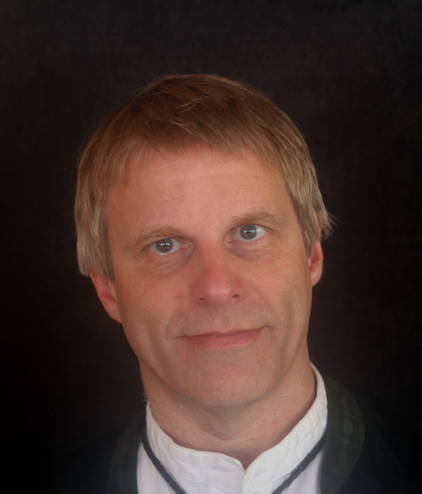
\includegraphics[width=\textwidth]{tononi}
				\end{figure}
			\end{column}
		\end{columns}
		Основные публикации:
		\nocite{*}
		\printbibliography[keyword={tononi}]
		
	
	\end{frame}
	
	\begin{frame}
		\frametitle{Теория интегрированной информации (IIT)}
		
		\begin{columns}
			\begin{column}{0.9\textwidth}
				\nocite{*}
				\printbibliography[keyword={iit}]
			\end{column}
			\begin{column}{0.1\textwidth}
				\begin{figure}
					
\includegraphics[width=\textwidth]{logo}
				\end{figure}
			\end{column}
		\end{columns}

		\begin{itemize}
			\item Разрабатывается с 2004 года
			\item Цель: создать теоретический подход, обладающий объясняющей и предсказывающей силой
			\item Основные вопросы:
				\begin{itemize}
					\item почему сознание генерируется кортико-таламической системой, а не мозжечком?
					\item почему сознание исчезает во время сна, хотя мозг активен?
					\item почему теряется сознание во время конвульсий, хотя нейронная активность высокая и синхронная?
					\item почему нет прямого вклада нейронной активности в сознание, хотя доказано, что она влияет на содержание переживания (experience)?
				\end{itemize}
			\item \href{http://integratedinformationtheory.org/}{Сайт с демонстрациями}
		\end{itemize}		
	\end{frame}	


	\begin{frame}
		\frametitle{Сложные вопросы}
		
		Только теория может ответить на сложные вопросы:
		\begin{itemize}
			\item  Обладает ли новорожденный сознанием? В какой степени?
			\item Обладает ли сознанием пациент с остаточной нейронной активностью в одной из областей коры?
			\item Обладают ли сознанием интеллектуальные машины, способные отлично распознавать изображения и отвечать на сложные вопросы?
		\end{itemize}
		\par\bigskip
		\textbf{Нужно двигаться от феноменологии, от основных принципов, к тому, как они реализуются физическими системами, а не от нейронных механизмов к условиям, при которых на их основе возникает сознание.}
	\end{frame}		
	
	\begin{frame}
		\frametitle{Аксиомы}
		
		Самоочевидные (по Декарту) истины о сознании:
		\begin{itemize}
			\item \textit{существование}: <<Я переживаю, значит я существую>>, 
			\item \textit{структурированность}: переживания характеризуются несколькими аспектами в разных сочетаниях (голубой квадрат справа),
			\item \textit{информативность}: одно переживание может быть отличено от другого переживания, 
			\item \textit{интегрированность}: переживание строго не разделимо на независимые части (красный треугольник),
			\item \textit{единственность}: одно переживание исключает наличие других в то же самое время, т.е. обладает определенными пространственно-временными разрешением.
		\end{itemize}
	\end{frame}

	\begin{frame}
		\frametitle{Постулаты}
		
		Недоказуемые предположения о физическом субстрате сознания.
		\par\bigskip
		Постулаты, относящиеся к свойствам физических систем (механизмов):
		\begin{itemize}
			\item \textit{существование}: системы существуют в определенном состоянии, система состоит из подсистем, 
			\item \textit{структурированность}: элементарные подсистемы могут быть объединены в системы более высокого порядка. 
		\end{itemize}
	\end{frame}

	\begin{frame}
		\frametitle{Постулаты}
		
		Постулаты, характеризующие элементы системы или подсистемы:
		\begin{itemize}
			\item \textit{информативность}: подсистема вносит вклад в сознательное переживание (генерирует информацию), если она ограничивает множество состояний системы, ее причинно-следственный репертуар (определяет <<имеющие значение отличия>>),
			\item \textit{интегративность}: подсистема вносит вклад в сознание, если она определяет причинно-следственный репертуар, неразделимый на независимые компоненты,
			\item \textit{единственность}: подсистема вносит вклад в сознание, если она определяет \textit{не более чем один} причинно-следственный репертуар, имеющий максимальное значение интеграции $\phi^{Max}$ и называющийся максимально несократимым причинно-следственным репертуаром (MICE) (в этом случае подсистема образует \textit{концепт}). 
		\end{itemize}
	\end{frame}

	\begin{frame}
		\frametitle{Постулаты}
		
		Постулаты, характеризующие систему в целом:
		\begin{itemize}
			\item \textit{информативность}: множество элементов системы обладает сознанием, если соответствующие им подсистемы определяют <<имеющие значение отличия>>, т.е. образуют концептуальную структуру (<<созвездие>> точек в пространстве связанных прошлых и будущих состояний системы),
			\item \textit{интегративность}: множество элементов системы обладает сознанием, если соответствующие им подсистемы определяют несократимую концептуальную структуру (интеграция $\Phi$ оценивается путем разделения элементов на подмножества однонаправленными разрезами),
			\item \textit{единственность}: среди всех пересекающихся множеств элементов, только одно множество может обладать сознанием: то, которое определяет максимально несократимую концептуальную структуру (MICS, quale) (локальный максимум интегрированной информации $\Phi^{Max}$ называется \textit{комплексом}).
		\end{itemize}
	\end{frame}
	
	\begin{frame}
		\frametitle{Подсистема: матрица переходов}

		Подсистемой (механизмами) могут быть что угодно, что обладает каузальной ролью в некоторой системе: нейрон в мозге или логический вентиль в компьютере.
		
		\begin{figure}
			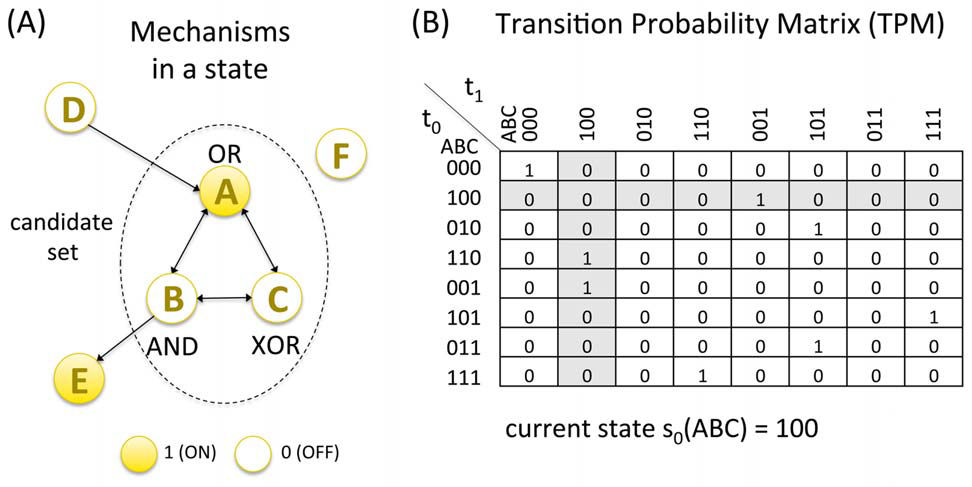
\includegraphics[width=0.7\textwidth]{mechanisms}
		\end{figure}
	\end{frame}
				
	\begin{frame}
		\frametitle{Подсистема: структурированность}
		
		Подсистемы формируют системы второго порядка, которые, в свою очередь, составляют системы третьего порядка.
		
		\begin{figure}
			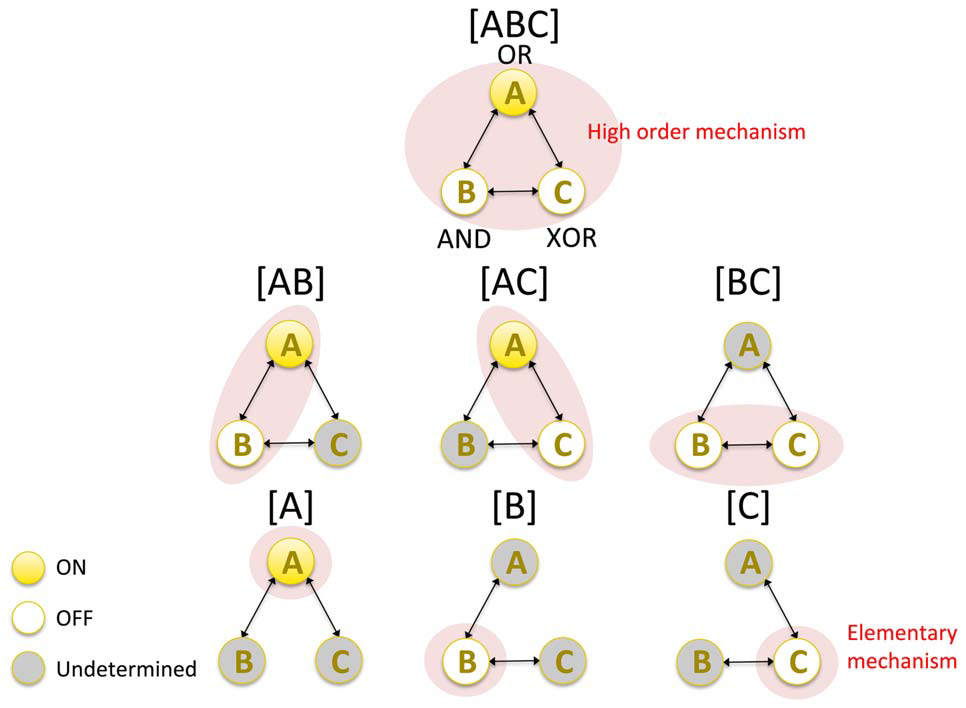
\includegraphics[width=0.7\textwidth]{composition}
		\end{figure}
	\end{frame}

	\begin{frame}
		\frametitle{Подсистема: информативность}
		
		Информация по Тонони предназначена для определения отличий, имеющих (<<внутреннее>>) значение в системе, что отличает ее от <<внешней>> информации по Шеннону.
		\par\bigskip
		Ограниченное элементом $A$ распределение прошлых (будущих) состояний системы $BCD$ (перспективы) называется причинным (следственным) репертуаром элемента $A$.
		
		\begin{figure}
			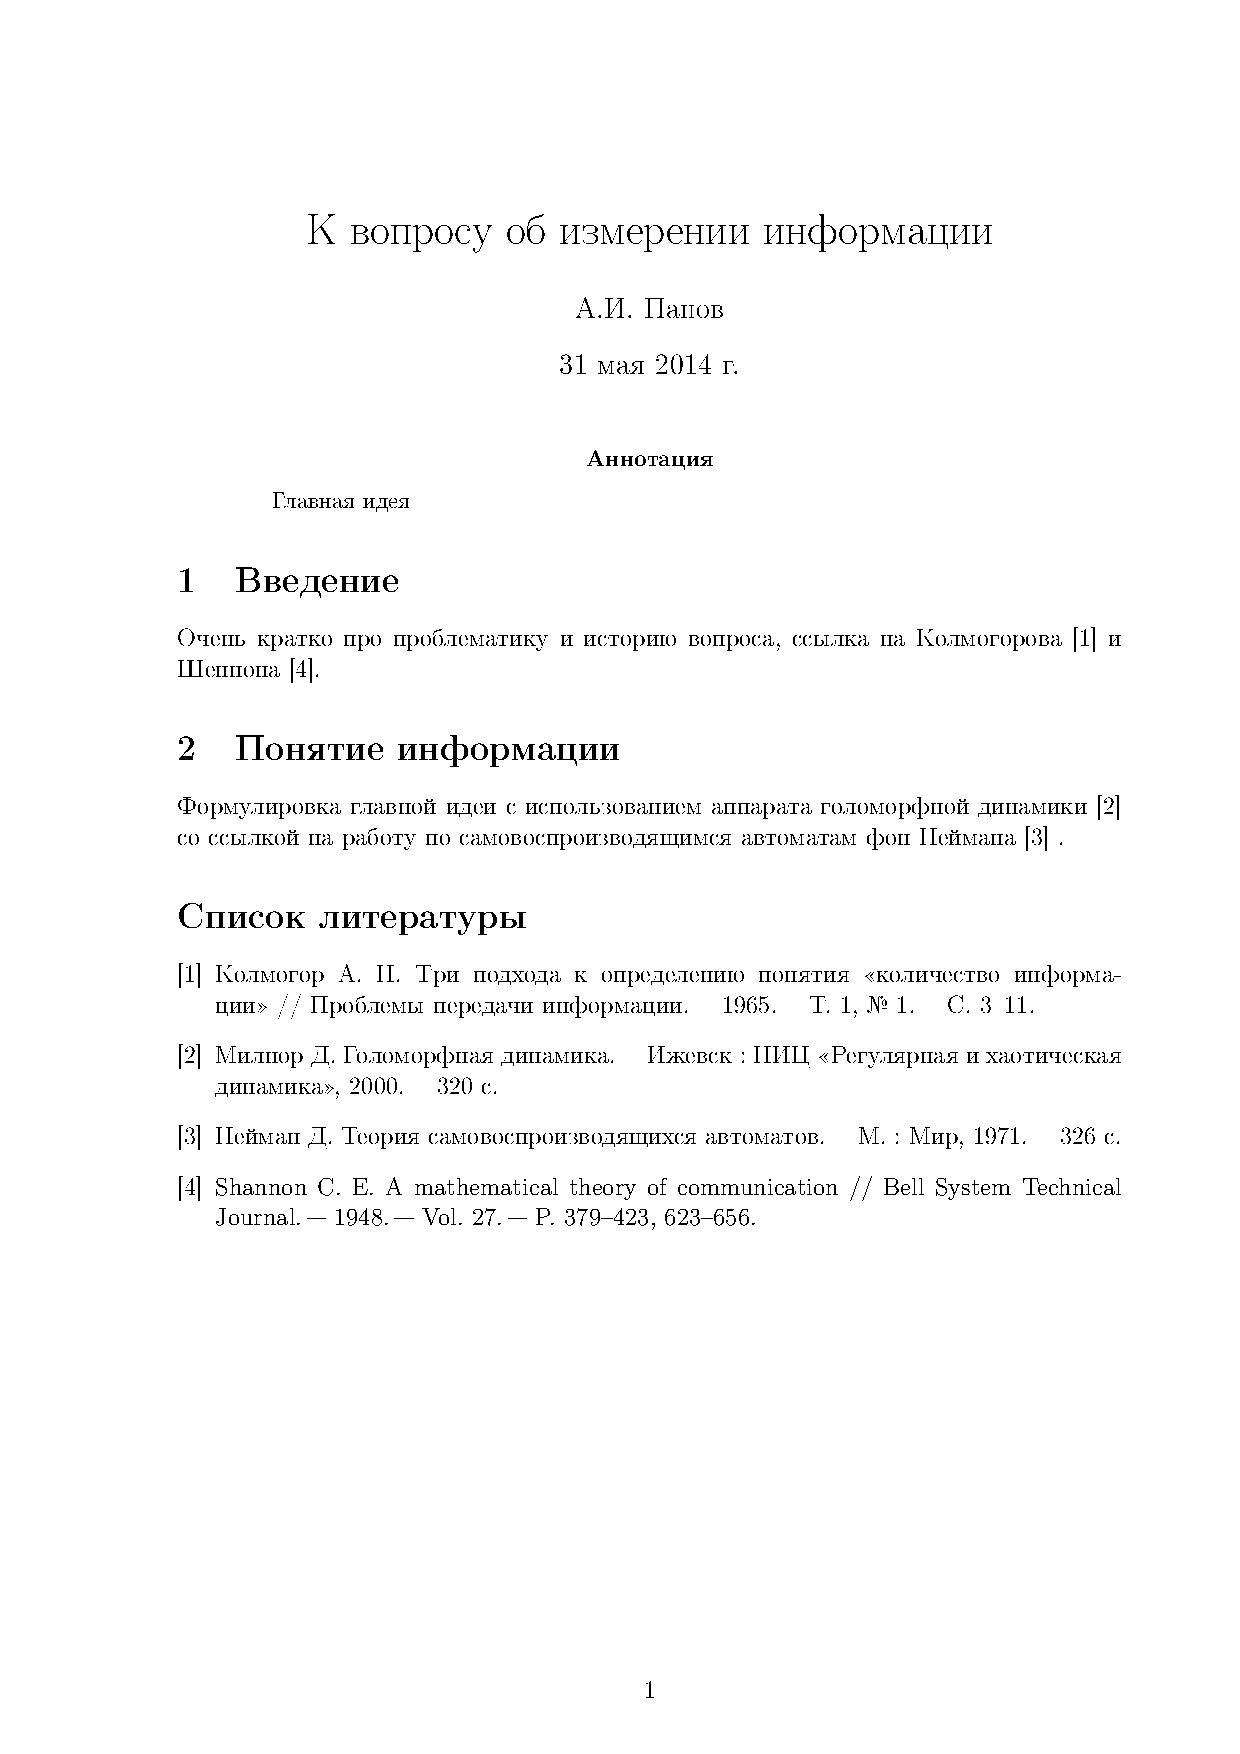
\includegraphics[width=0.8\textwidth]{information}
		\end{figure}
	\end{frame}
			
	\begin{frame}
		\frametitle{Подсистема: информативность}
		
		$ci,ce$ - причинная и следственная информации элемента $A=1$ относительно перспективы $ABC$.
		
		\begin{figure}
			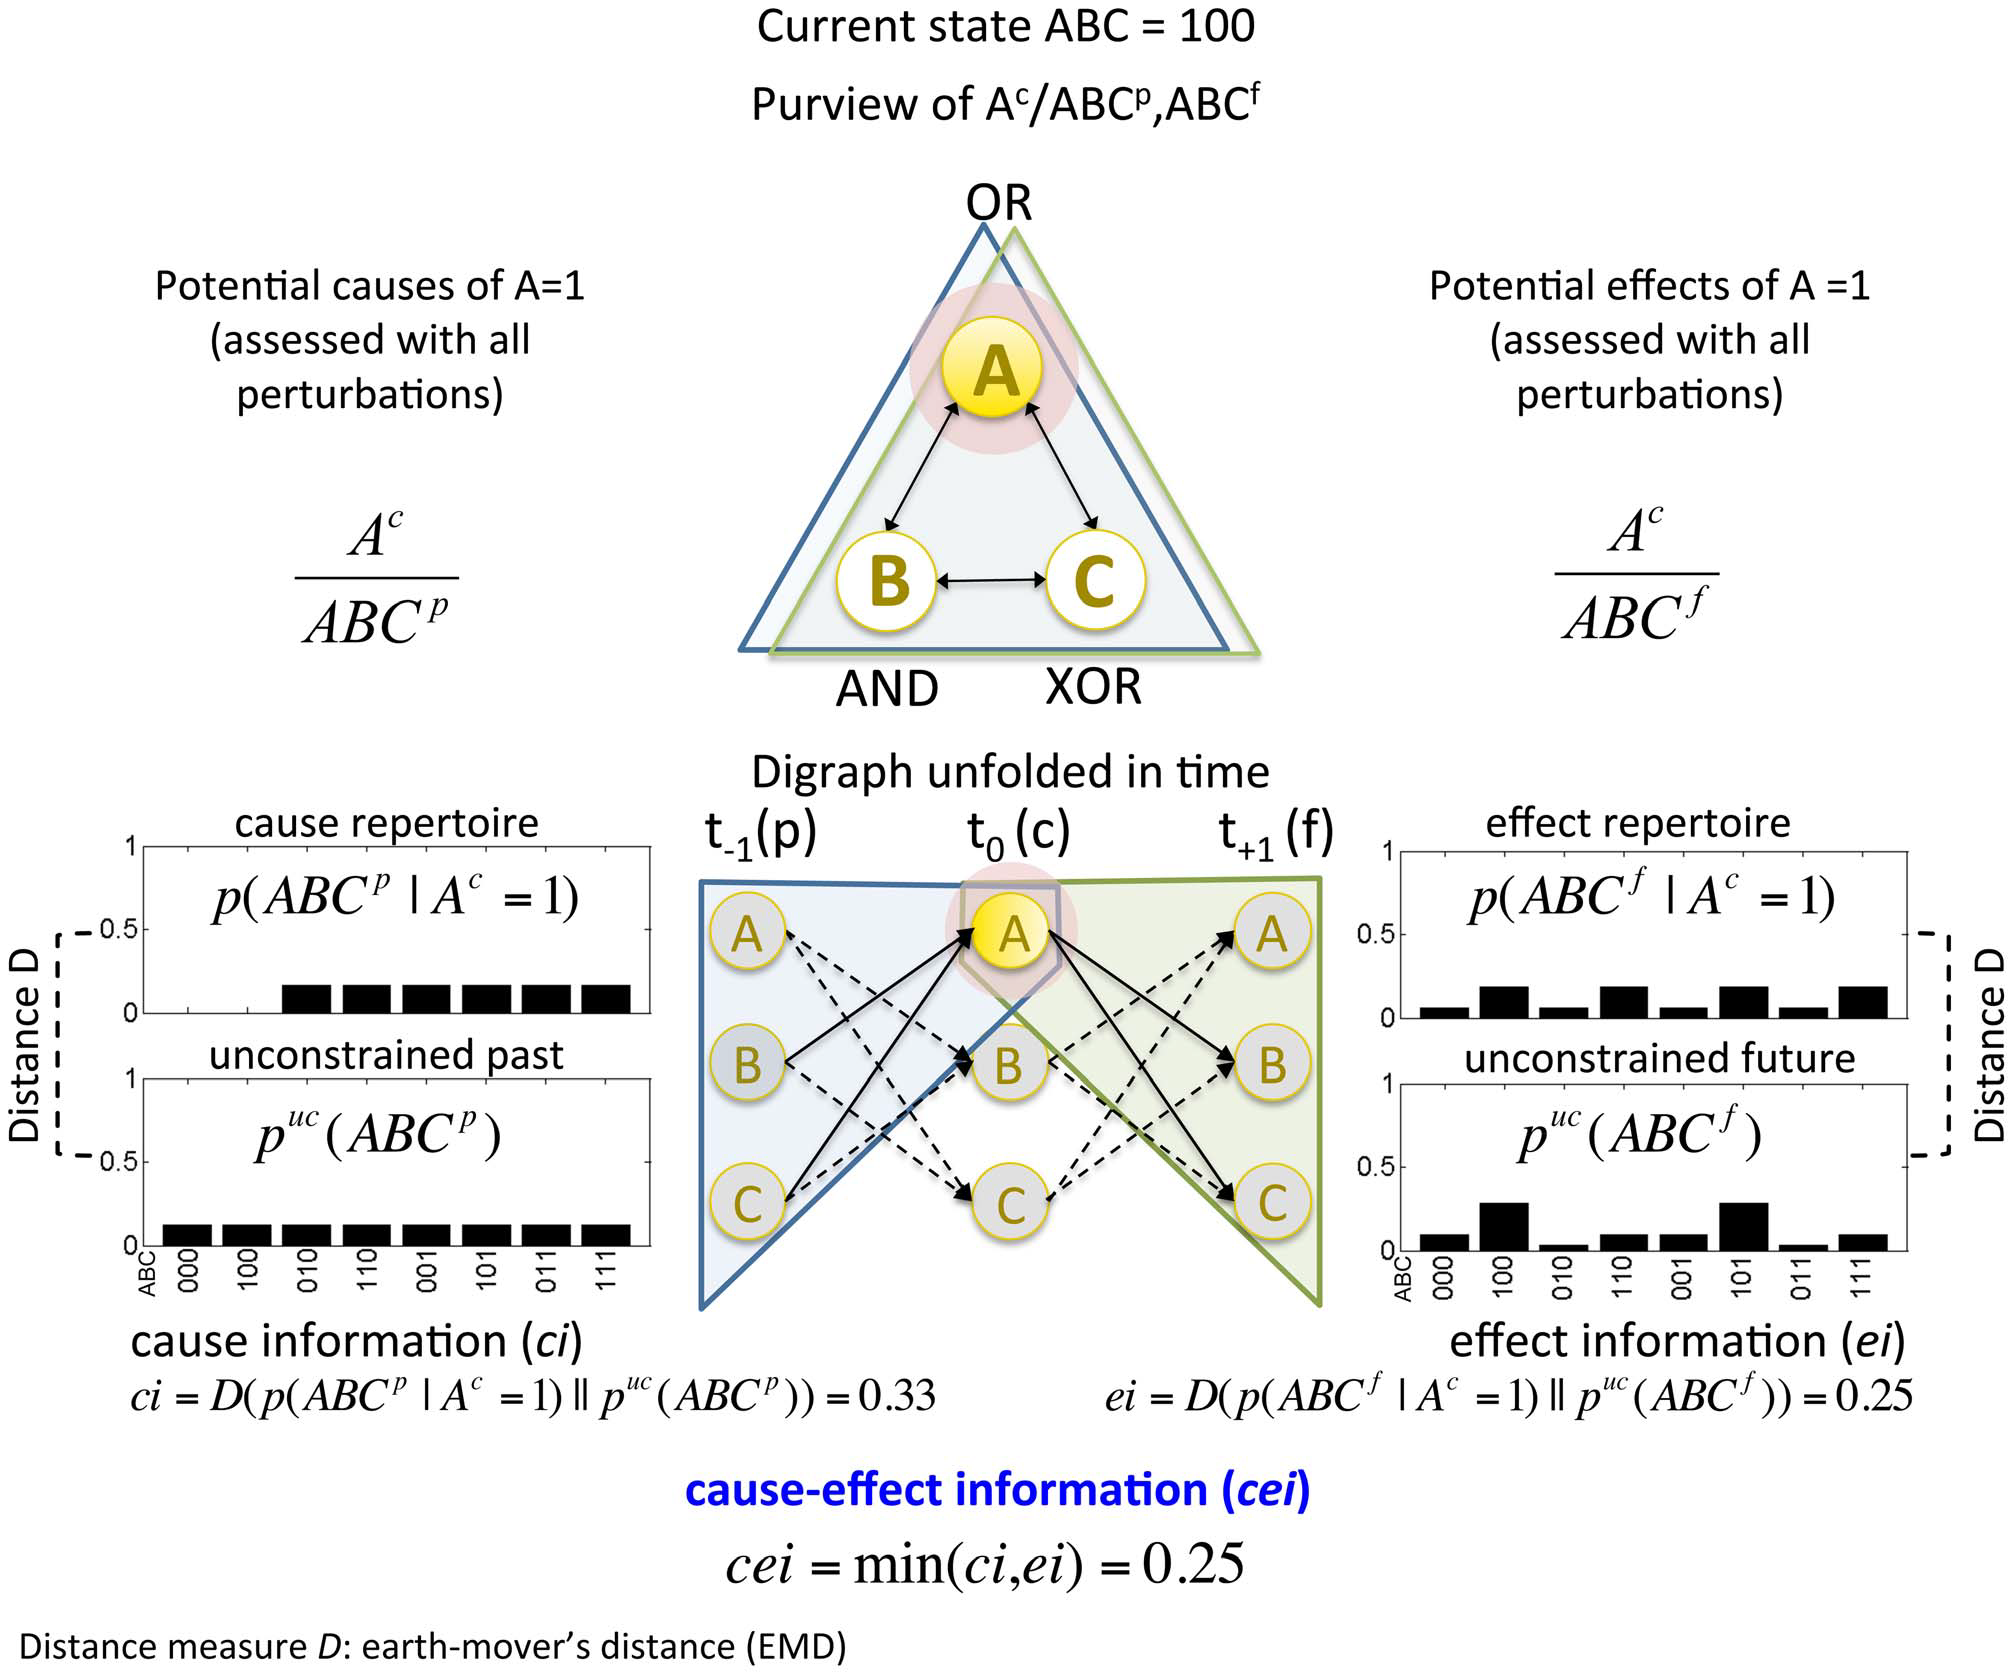
\includegraphics[width=0.6\textwidth]{causal}
		\end{figure}
	\end{frame}

	\begin{frame}
		\frametitle{Подсистема: интегративность}
		MIP - минимально информативное разделение.
		\begin{figure}
			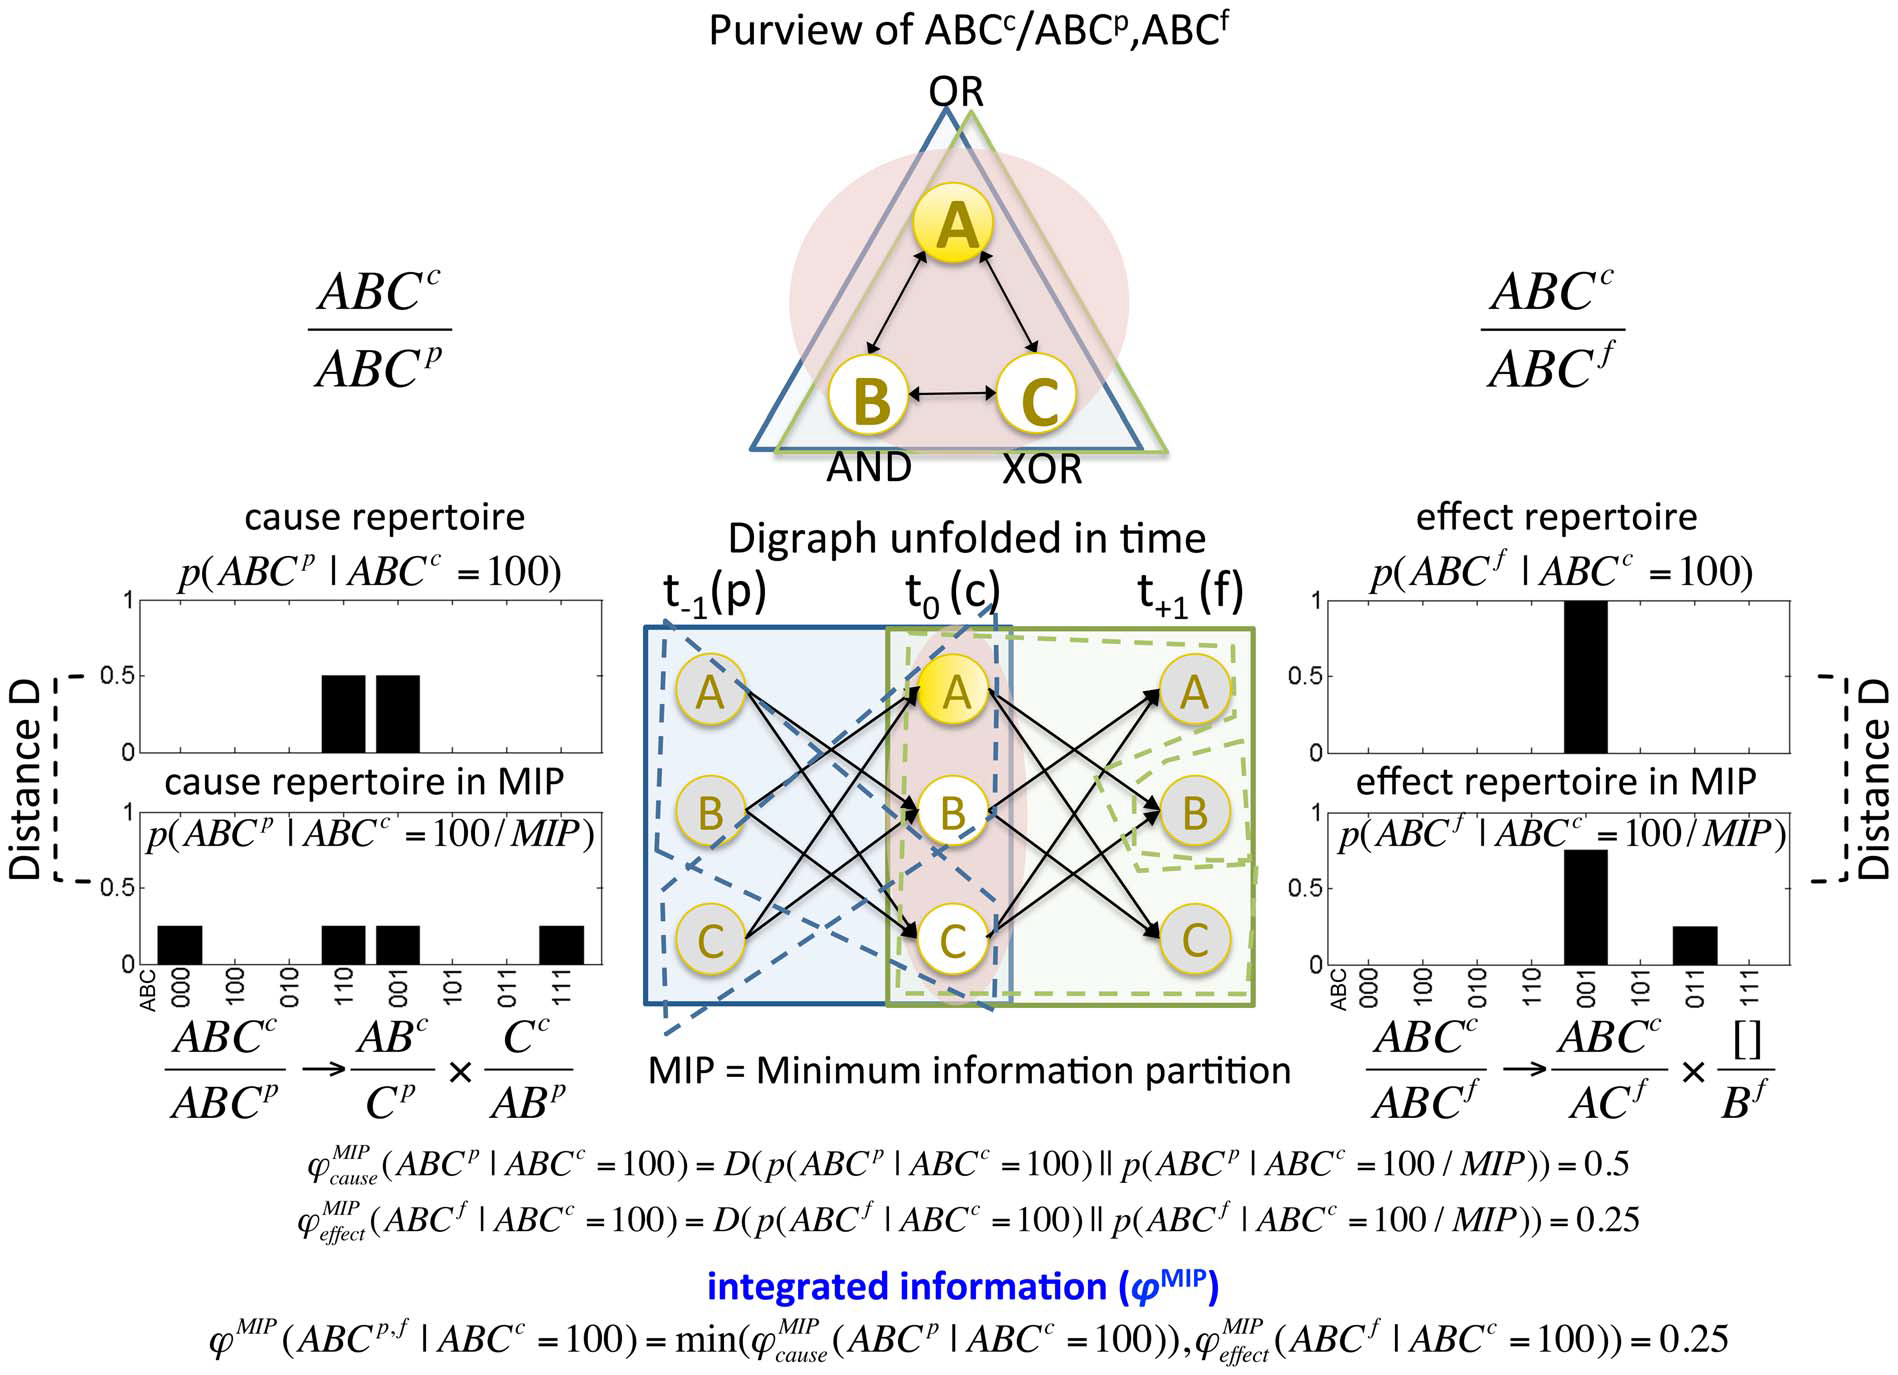
\includegraphics[width=0.8\textwidth]{integration}
		\end{figure}
	\end{frame}

	\begin{frame}
		\frametitle{Подсистема: интегративность}
		Подсистемы, не генерирующие информации, не существуют с внутренней точки зрения всей системы.
		\begin{figure}
			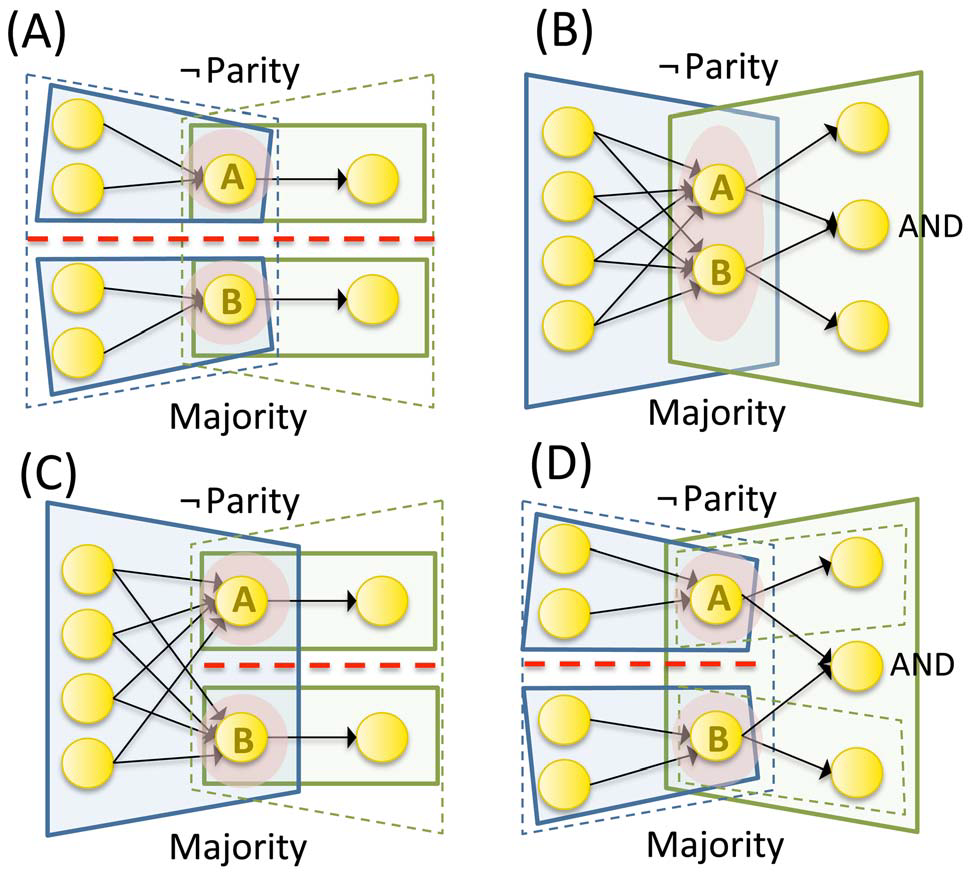
\includegraphics[width=0.5\textwidth]{existance}
		\end{figure}
	\end{frame}

	\begin{frame}
		\frametitle{Подсистема: единственность}
		
		Подсистема, определяющая максимально несократимый причинно-следственный репертуар (MICE) образует концепт.
		\par\bigskip
		<<Не следует множить причины без необходимости>> (каузальный вариант бритвы Оккама): только один набор синапсов может вызвать активность нейрона.
		
		\begin{columns}
			\begin{column}{0.5\textwidth}
				\begin{figure}
					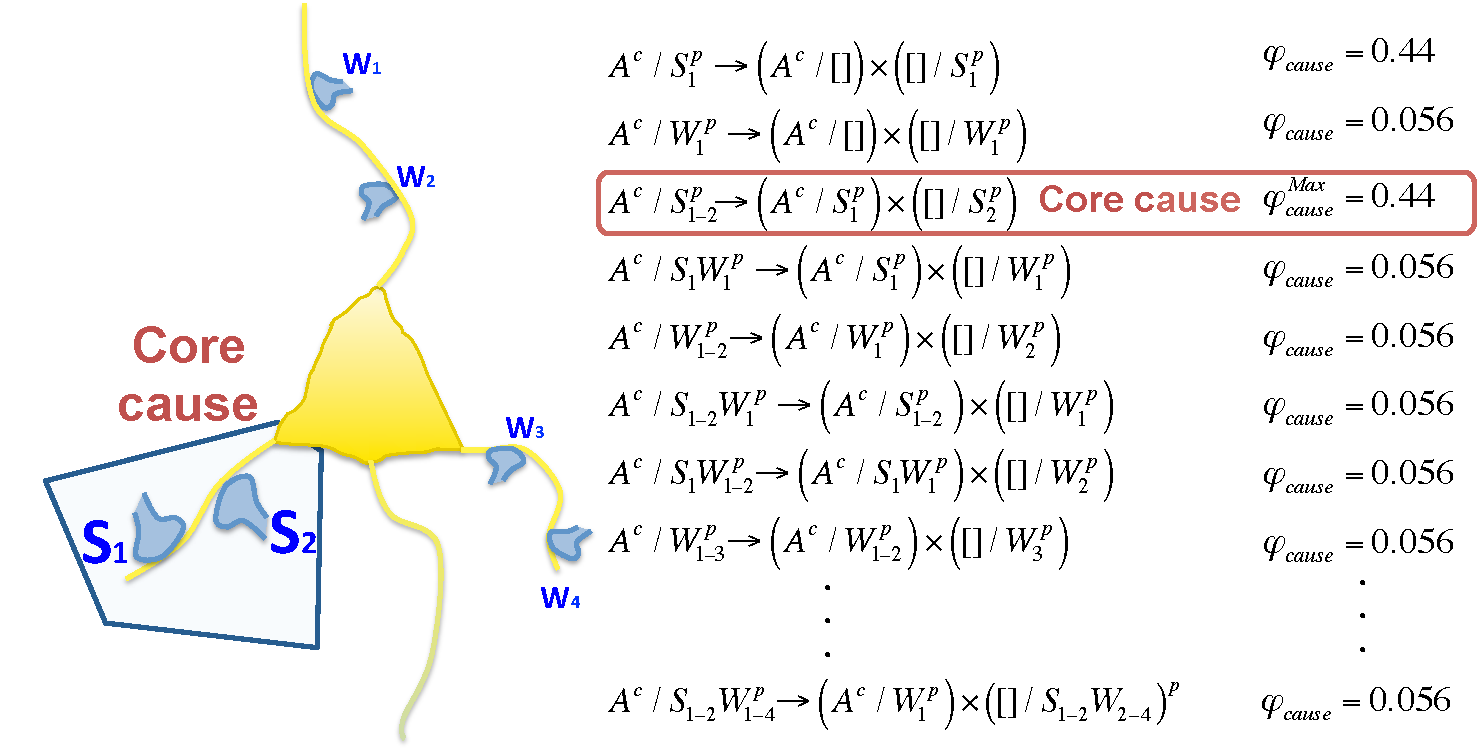
\includegraphics[width=\textwidth]{exc_neuron}
				\end{figure}				
			\end{column}
			\begin{column}{0.5\textwidth}
				\begin{figure}
					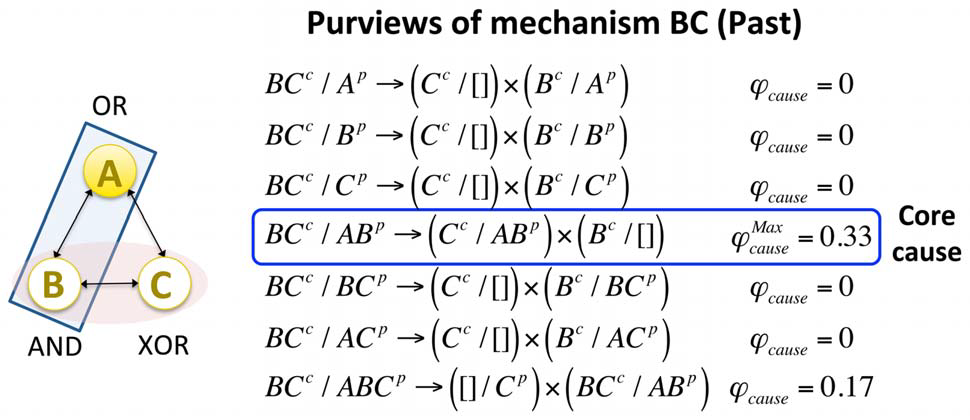
\includegraphics[width=\textwidth]{exclusion}
				\end{figure}
			\end{column}
		\end{columns}

	\end{frame}

	\begin{frame}
		\frametitle{Концепт}
		Максимально несократимый причинно-следственный репертуар (MICE) определяет, что такое концепт, а значение $\phi^{Max}$ определяет меру интеграции.
		\begin{figure}
			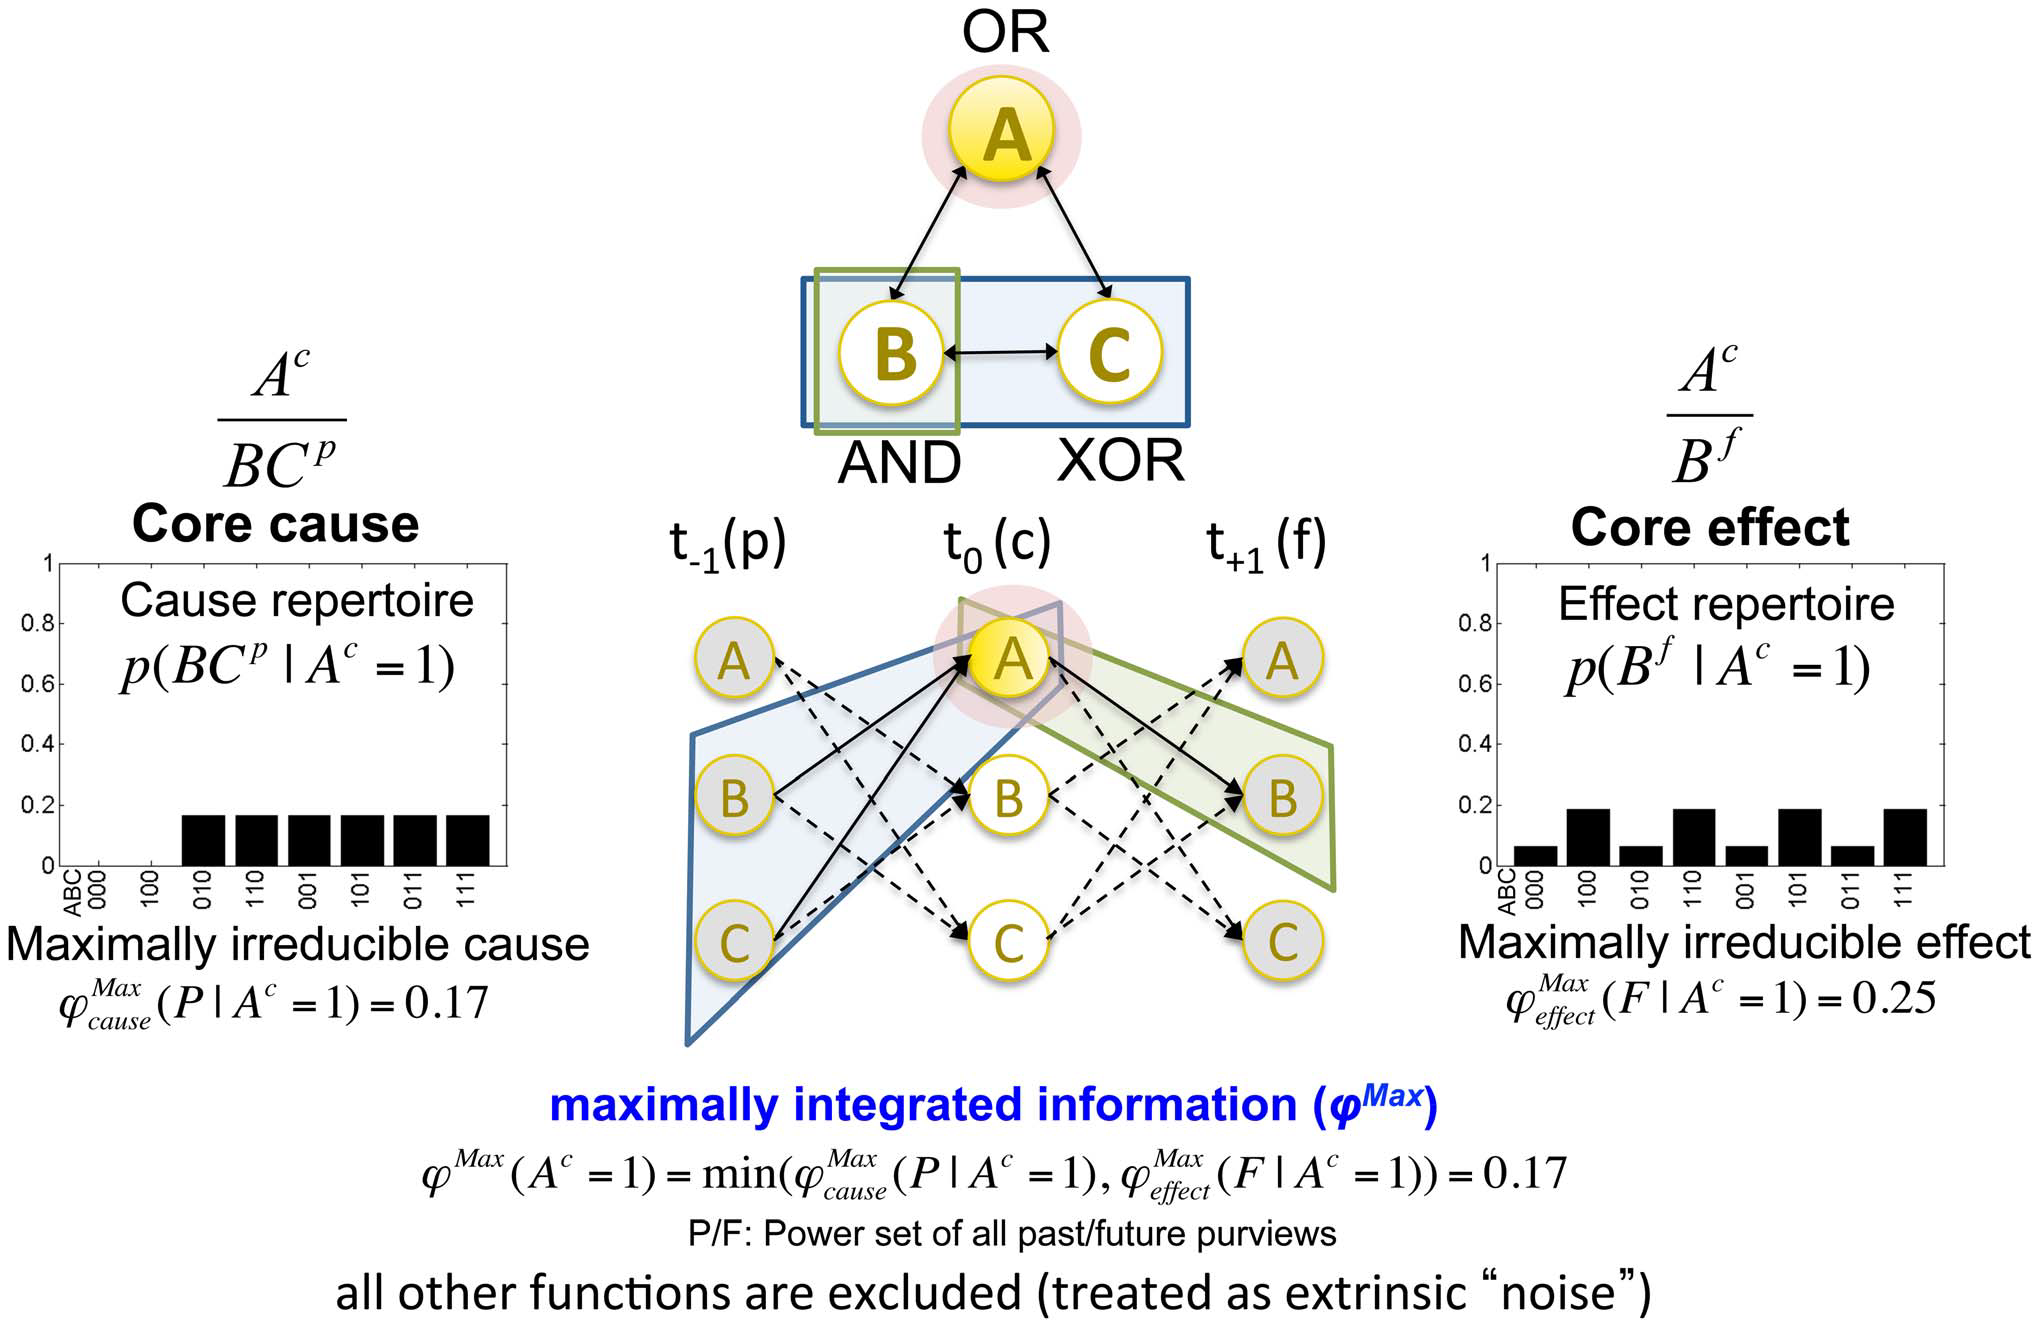
\includegraphics[width=0.7\textwidth]{concept}
		\end{figure}
	\end{frame}

	\begin{frame}
		\frametitle{Система: информативность}
		Множество всех концептов рассматриваемого множества образует его концептуальную структуру. Ось концептуального пространства соответствует одному из возможных сочетаний прошлого и будущего состояний системы.
		\begin{figure}
			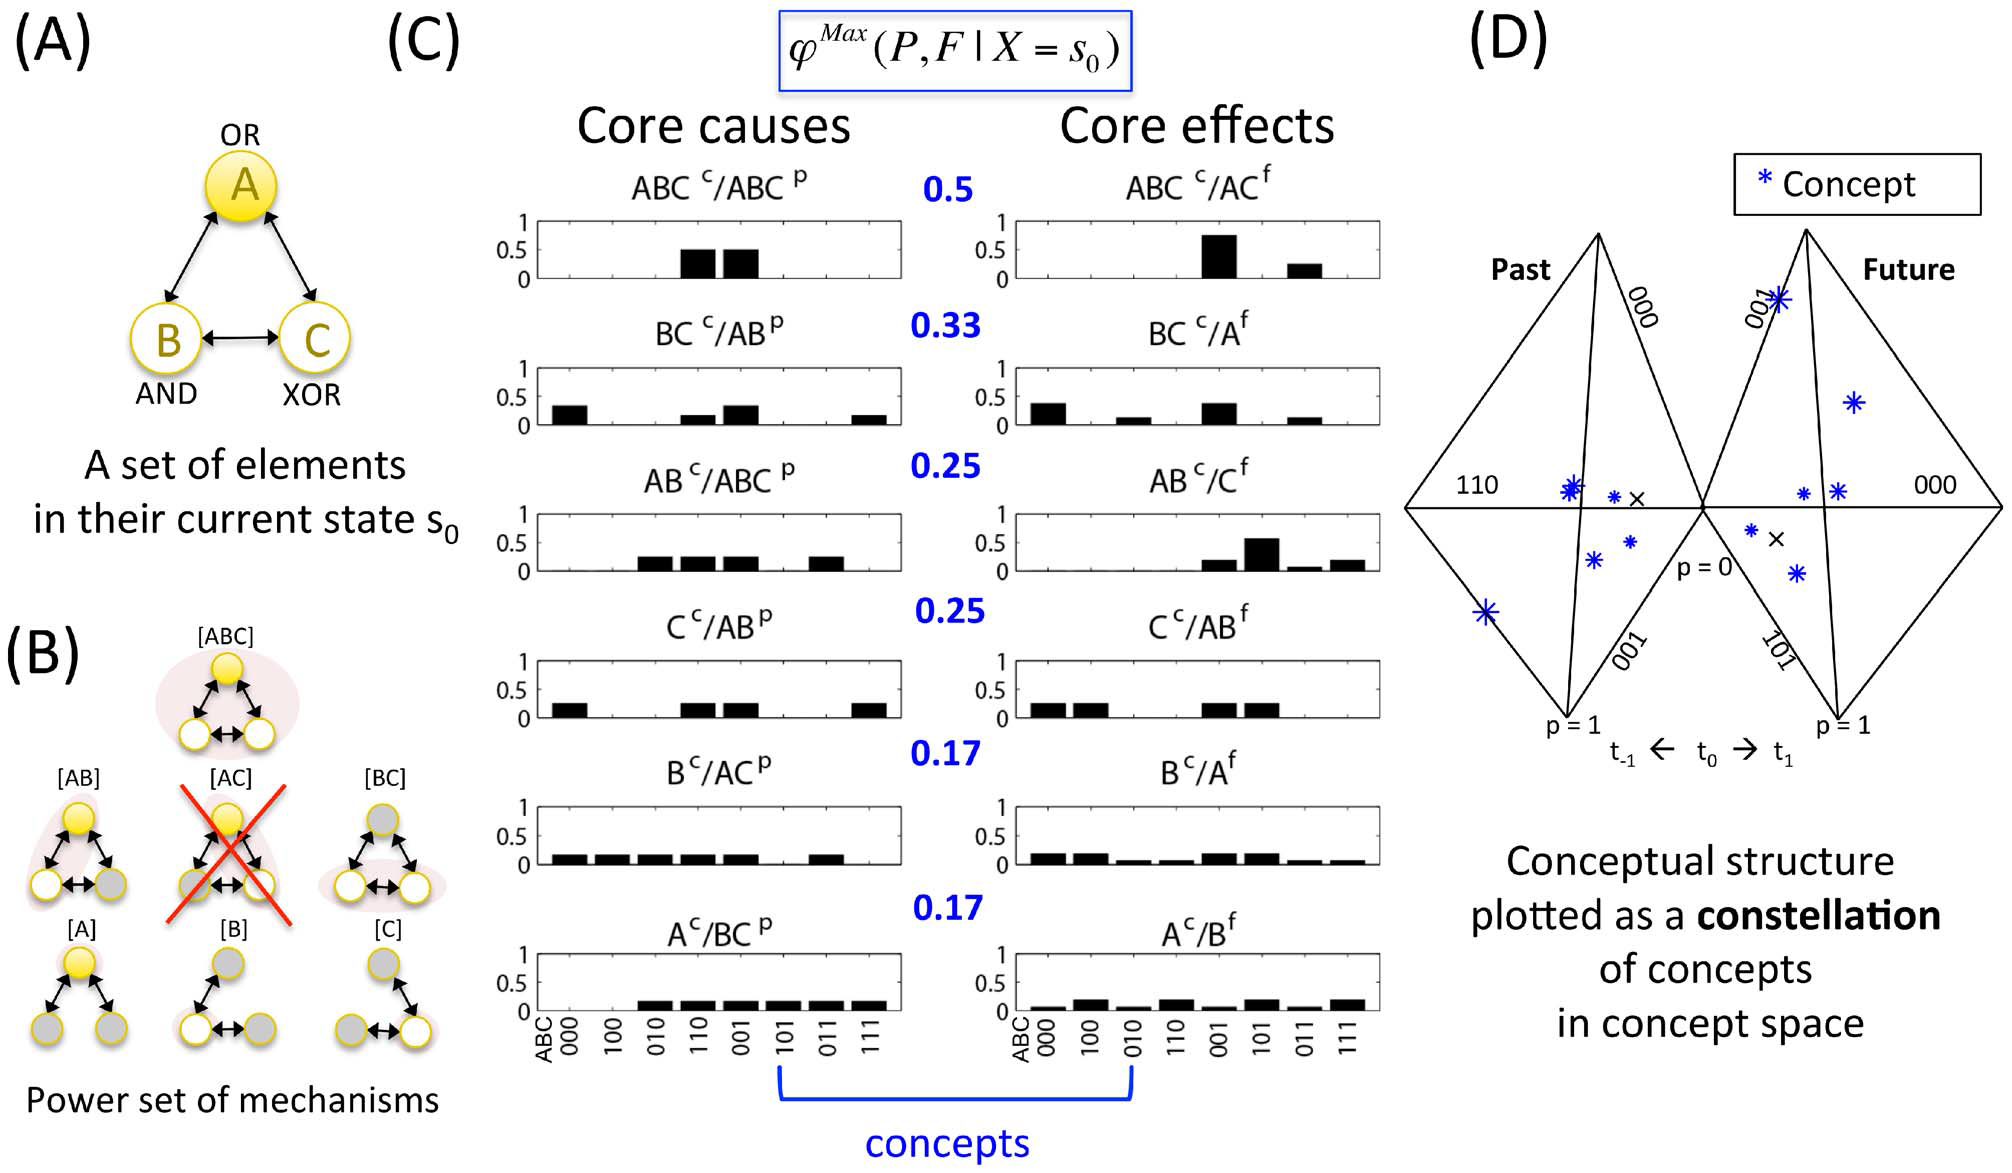
\includegraphics[width=0.8\textwidth]{system_info}
		\end{figure}
	\end{frame}

	\begin{frame}
		\frametitle{Система: информативность}

		\begin{figure}
			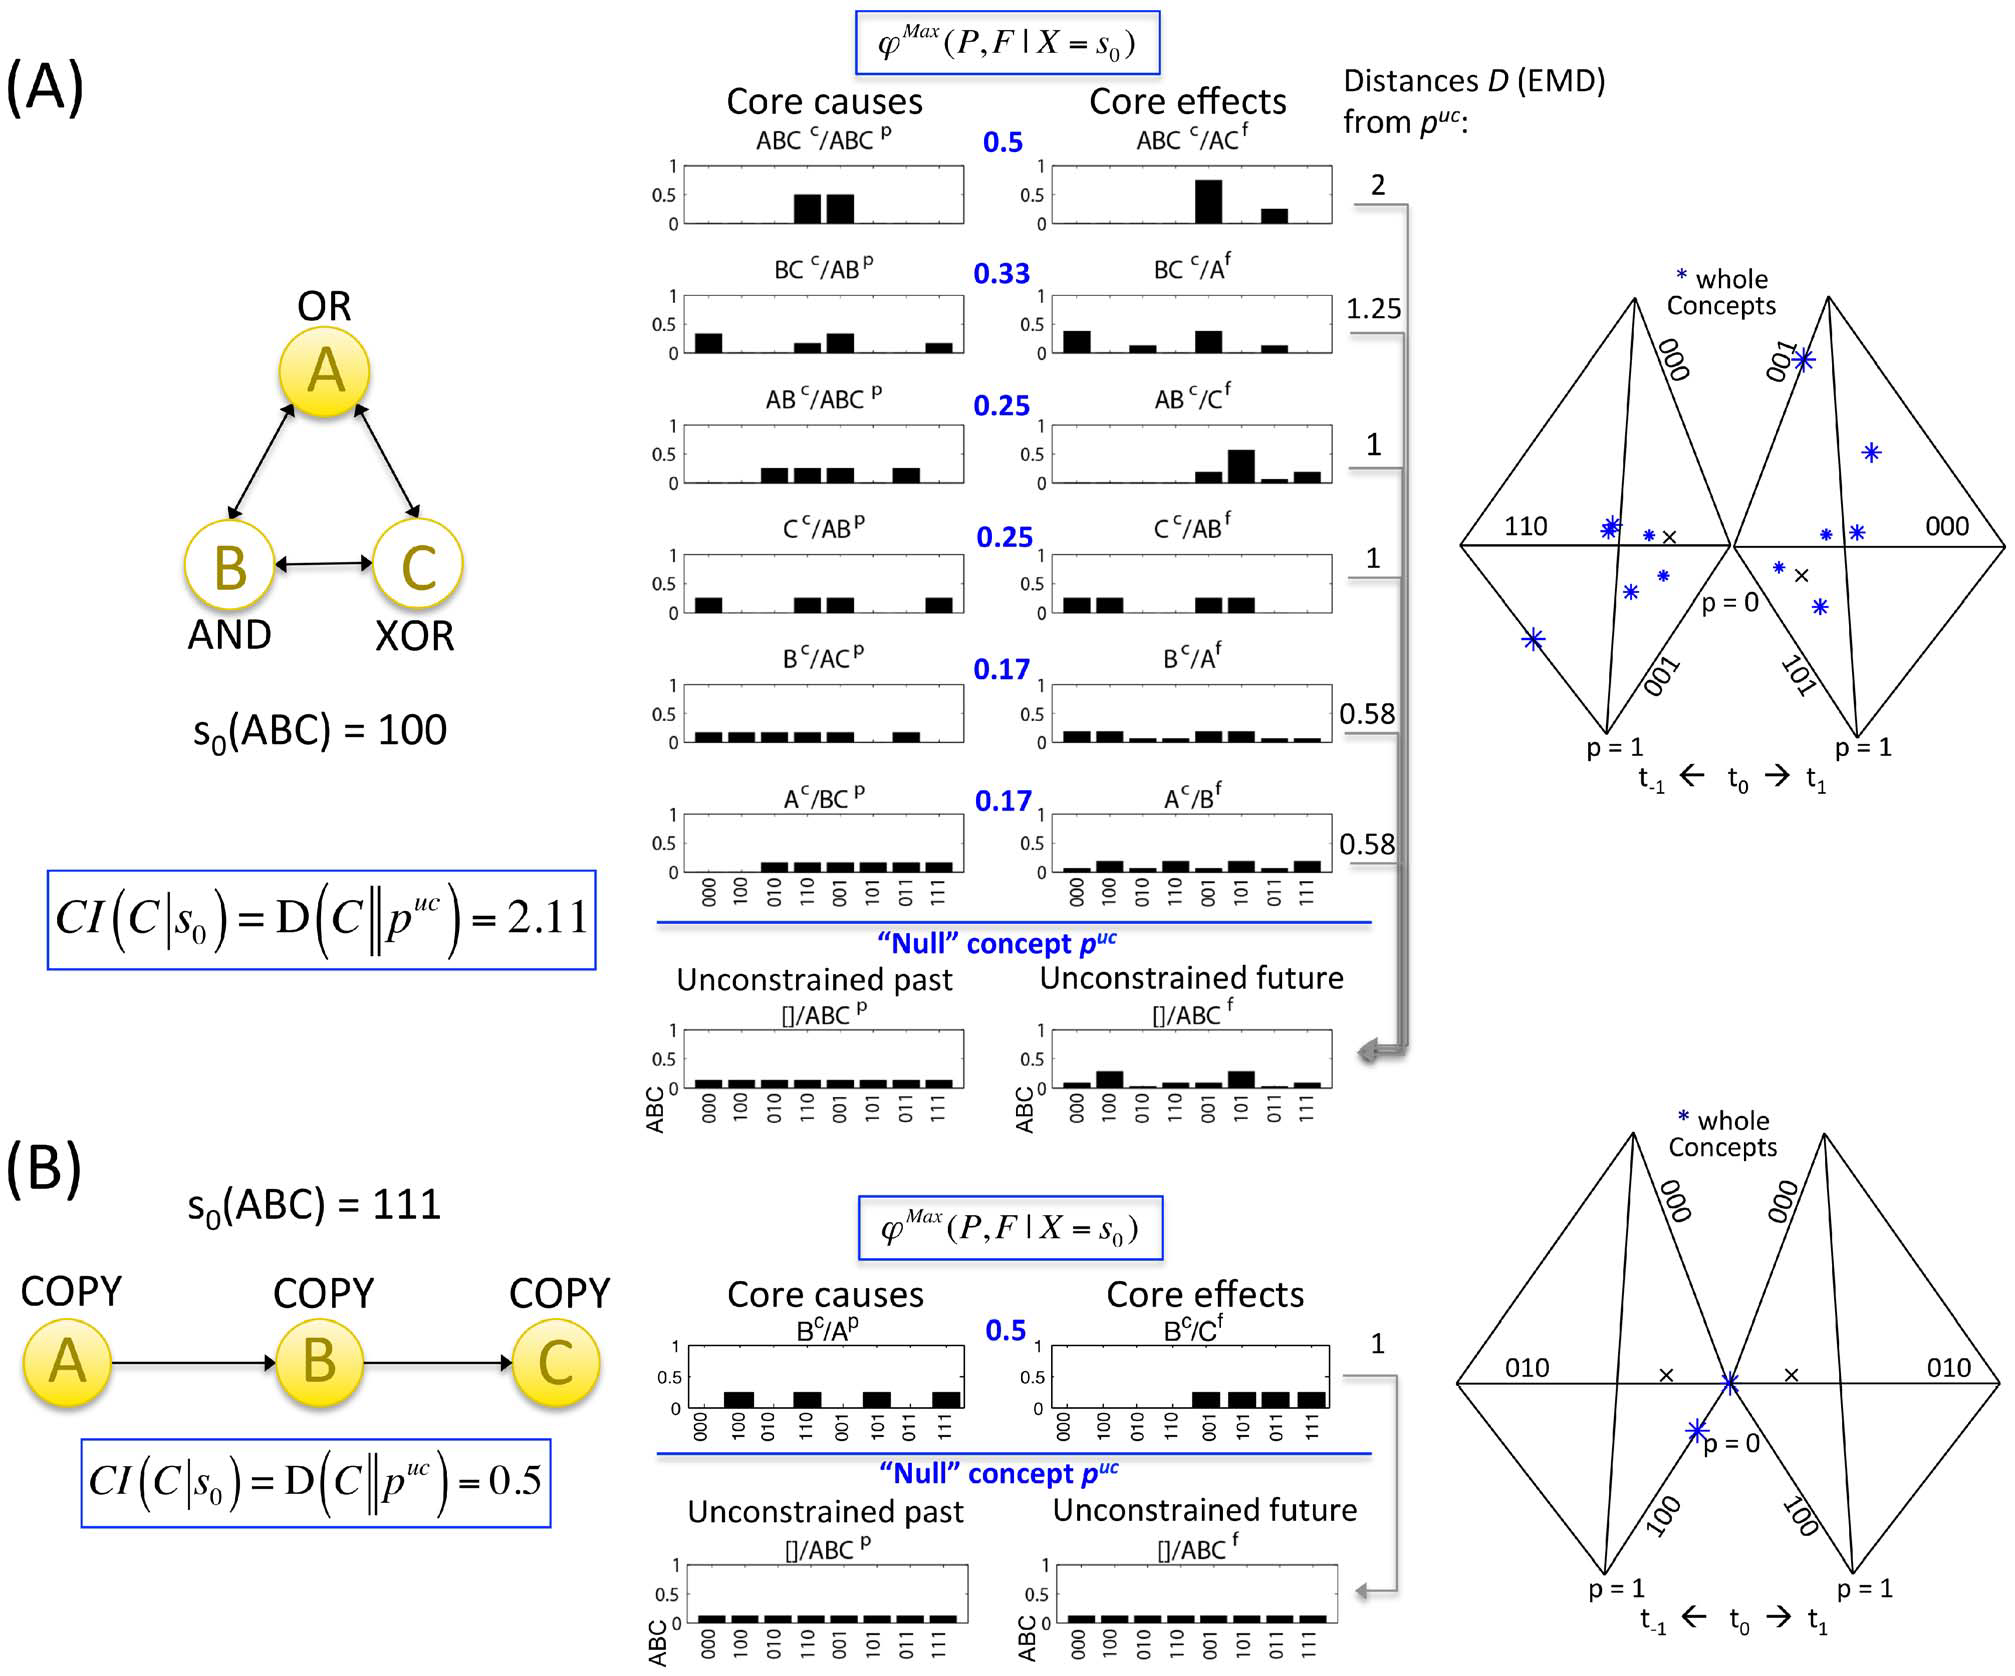
\includegraphics[width=0.75\textwidth]{system_ci}
		\end{figure}
	\end{frame}		
	
	\begin{frame}
		\frametitle{Система: интегративность}
		
		\begin{figure}
			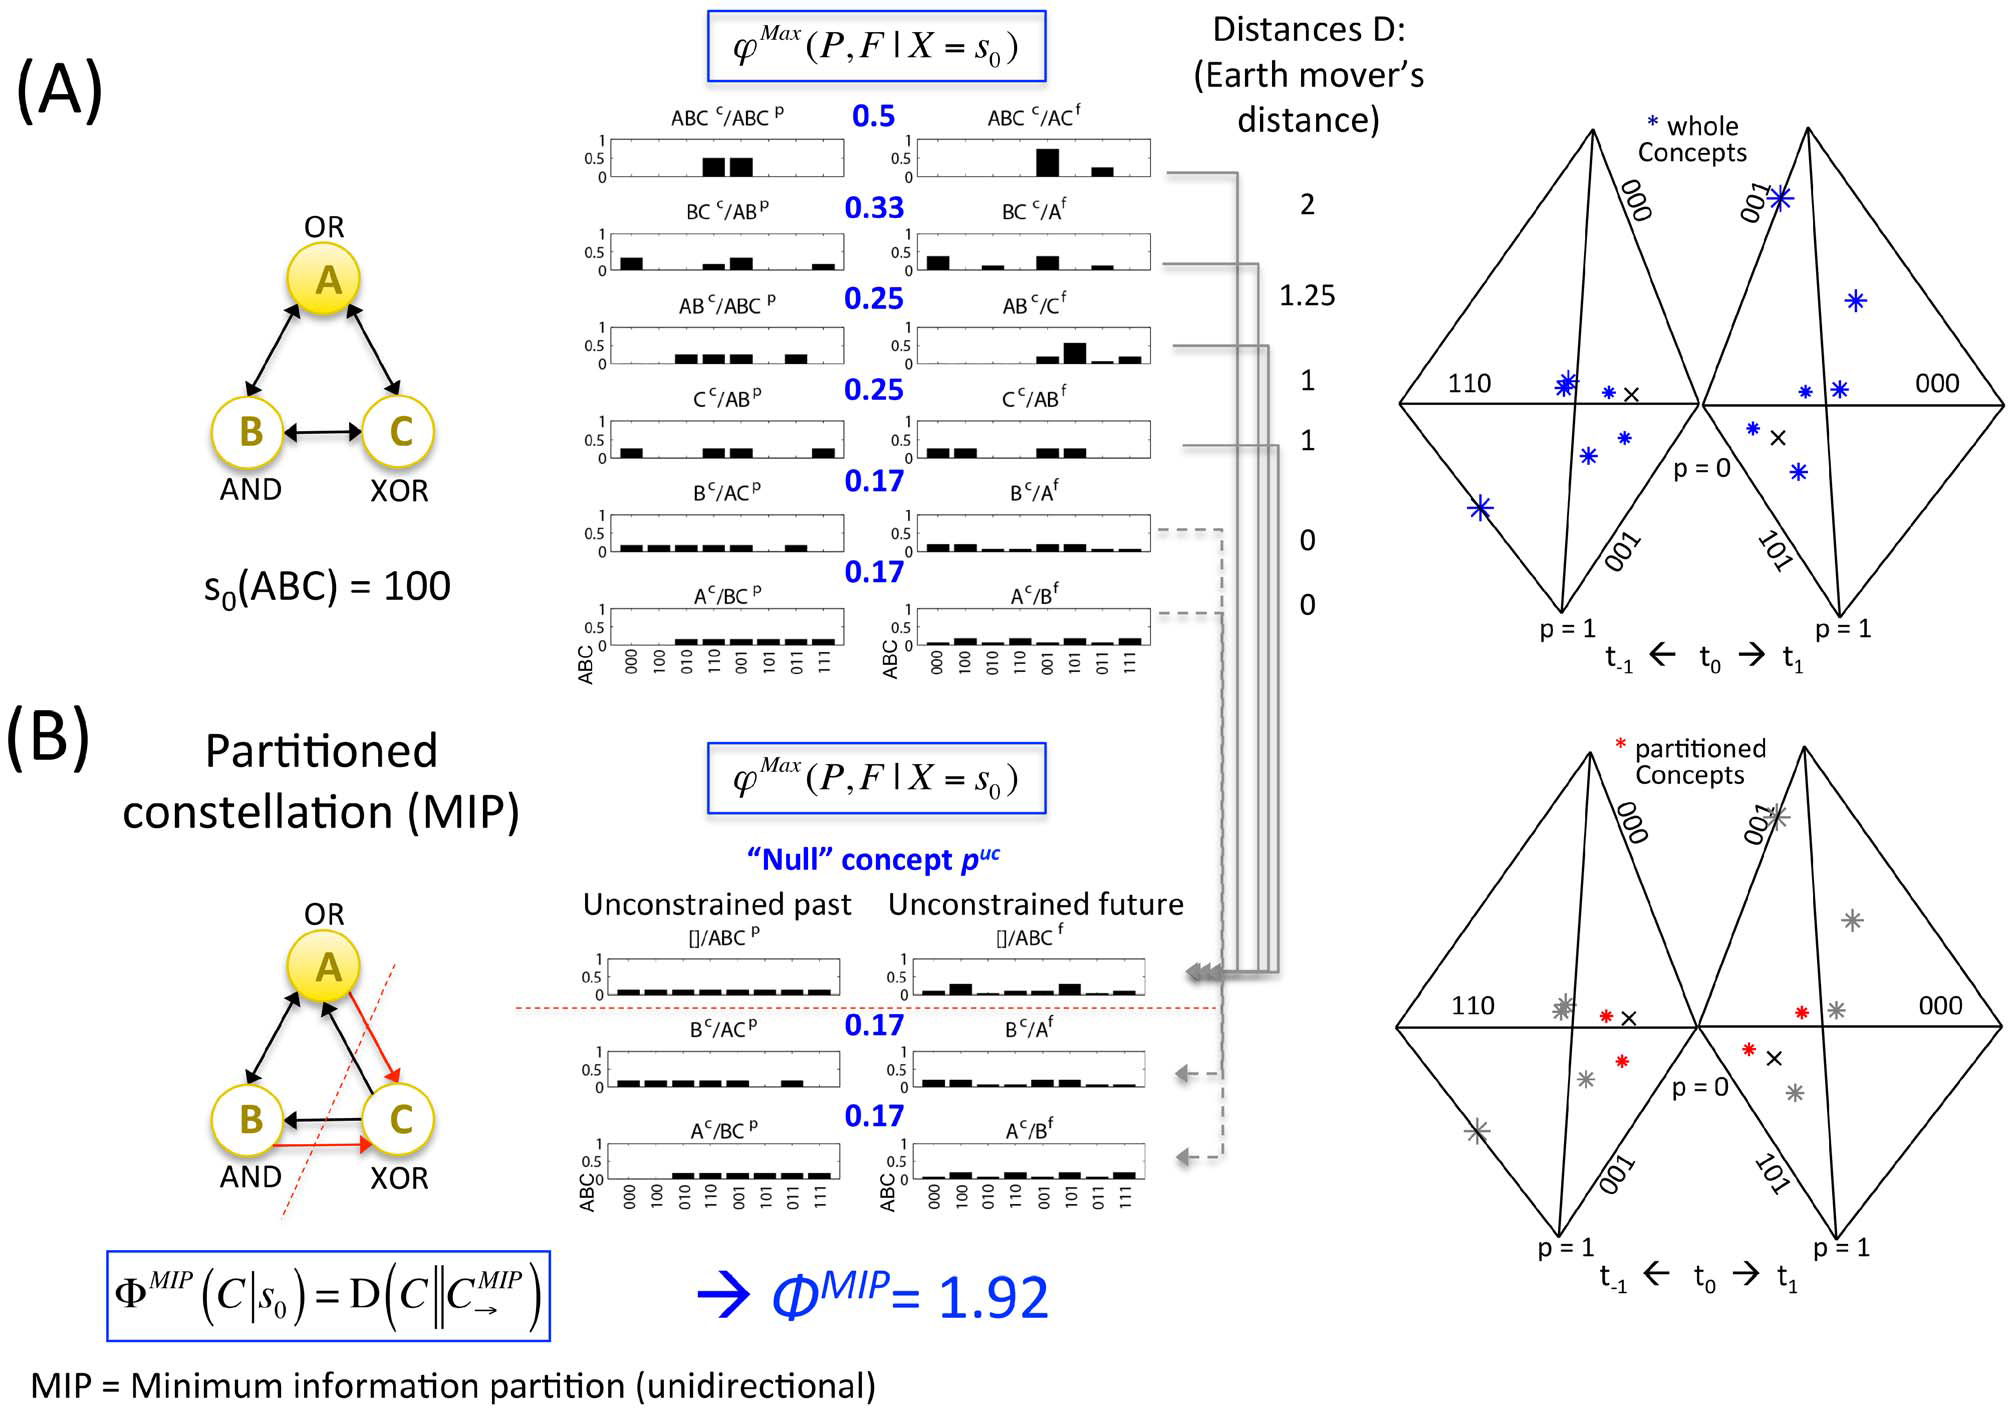
\includegraphics[width=0.9\textwidth]{system_integr}
		\end{figure}
	\end{frame}	
	
	\begin{frame}
		\frametitle{Система: интегративность}
		
		Множество элементов генерируют интегративную концептуальную информацию $\Phi$ только в том случае, если у него есть причины и эффекты в остальной части множества.
		\begin{figure}
			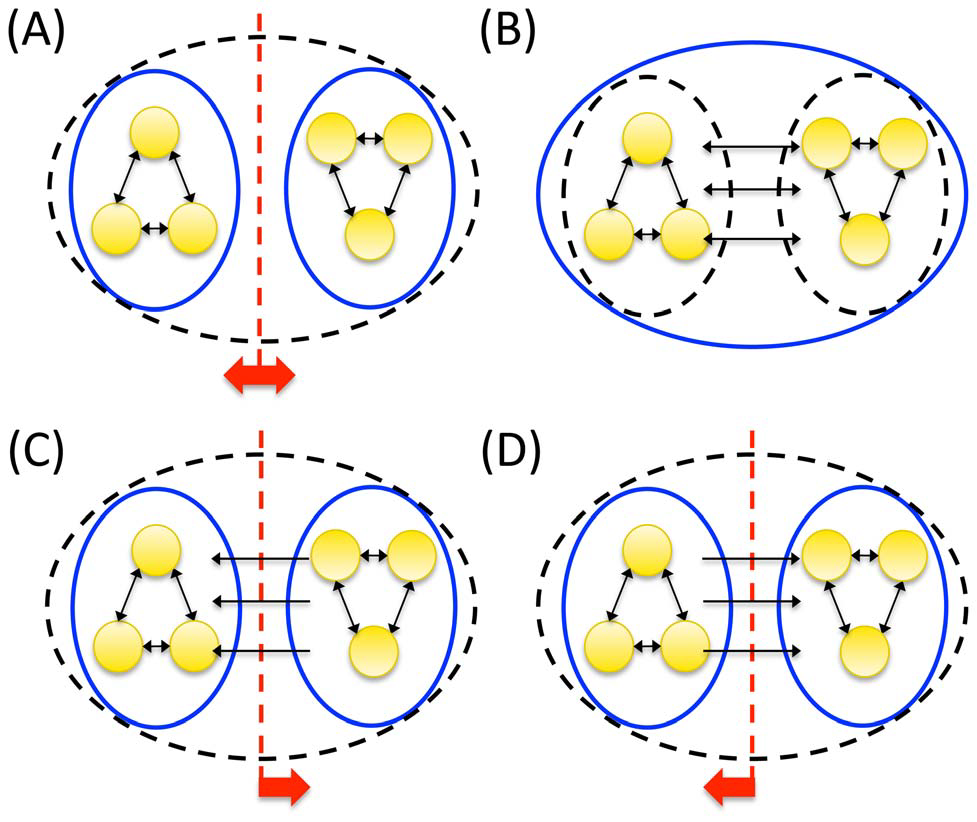
\includegraphics[width=0.5\textwidth]{system_exist}
		\end{figure}
	\end{frame}		
	
	\begin{frame}
		\frametitle{Система: единственность}
		
		При поиске максимально несократимой концептуальной структуры (MICS), рассматриваются все возможные подсистемы системы
		\begin{figure}
			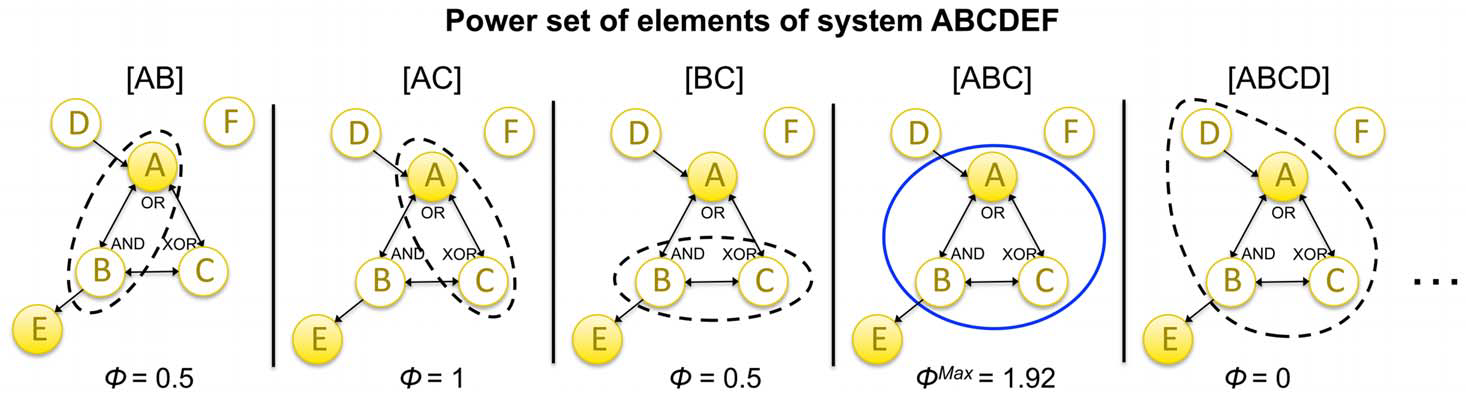
\includegraphics[width=\textwidth]{system_excl}
		\end{figure}
	\end{frame}	
	
	\begin{frame}
		\frametitle{Комплекс}
		
		Комплекс определяется как множество элементов в рамках системы, которая генерирует локальный максимум интегративной концептуальной информации $\Phi^{Max}$. Этот максимум рассматривается не только по элементам, но и по пространственно-временному разрешению.
		\begin{figure}
			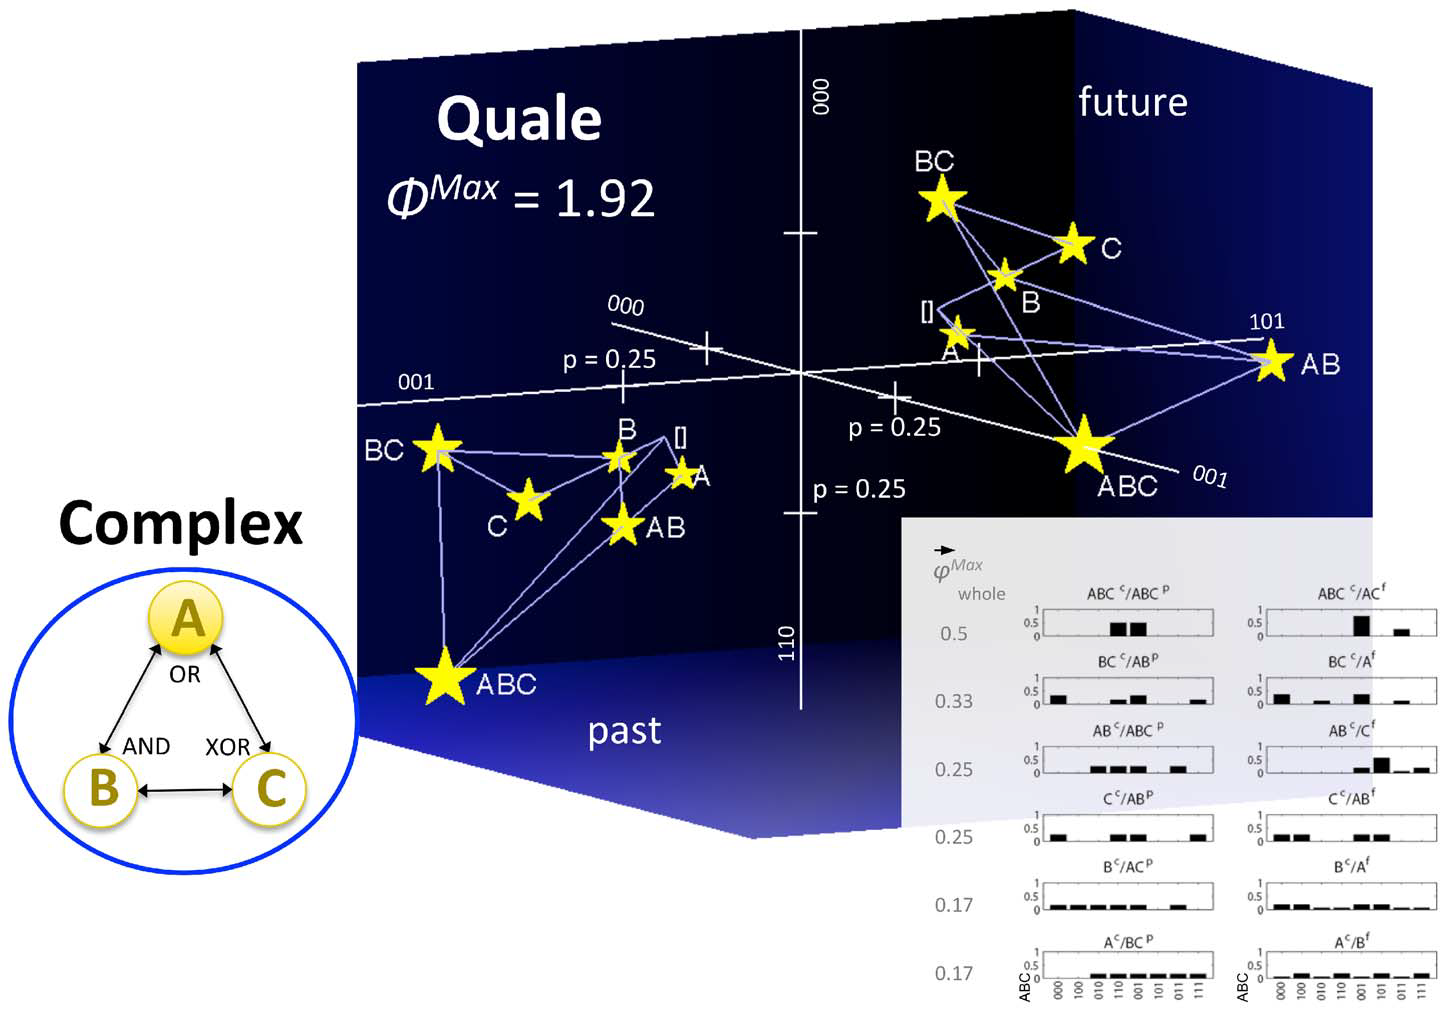
\includegraphics[width=0.5\textwidth]{complex}
		\end{figure}
	\end{frame}	
	
	\begin{frame}
		\frametitle{Центральное тождество}
		
		Переживание тождественно максимально несократимой концептуальной структуре (интегративной информационной структуре), определяемой подсистемами комплекса в некотором состоянии.
		\par\bigskip
		Количественно уровень сознания соответствует значению $\Phi^{Max}$, качество или содержание переживания соответствует определенному <<созвездию>> концептов, составляющих quale.
	\end{frame}	
		
	\begin{frame}
		\frametitle{Приложения и выводы}
		
		\begin{columns}
			\begin{column}{0.53\textwidth}
				\begin{itemize}
					\item Доминантный комплекс с наивысшим $\Phi^{Max}$ образуется меняющимся со временем множеством нейронов кортикальной системы и генерирует сознание бодрствования. 
					\item Наряду с этим комплексом есть несколько <<минимально осознанных>> побочных комплексов и много реактивных неосознанных процессов.
					\item При лоботомии могут образовываться два доминантных комплекса.
				\end{itemize}
				
			\end{column}
			\begin{column}{0.47\textwidth}
				Пример, когда система сводится к одному основному комплексу и нескольким побочным.
				\begin{figure}
					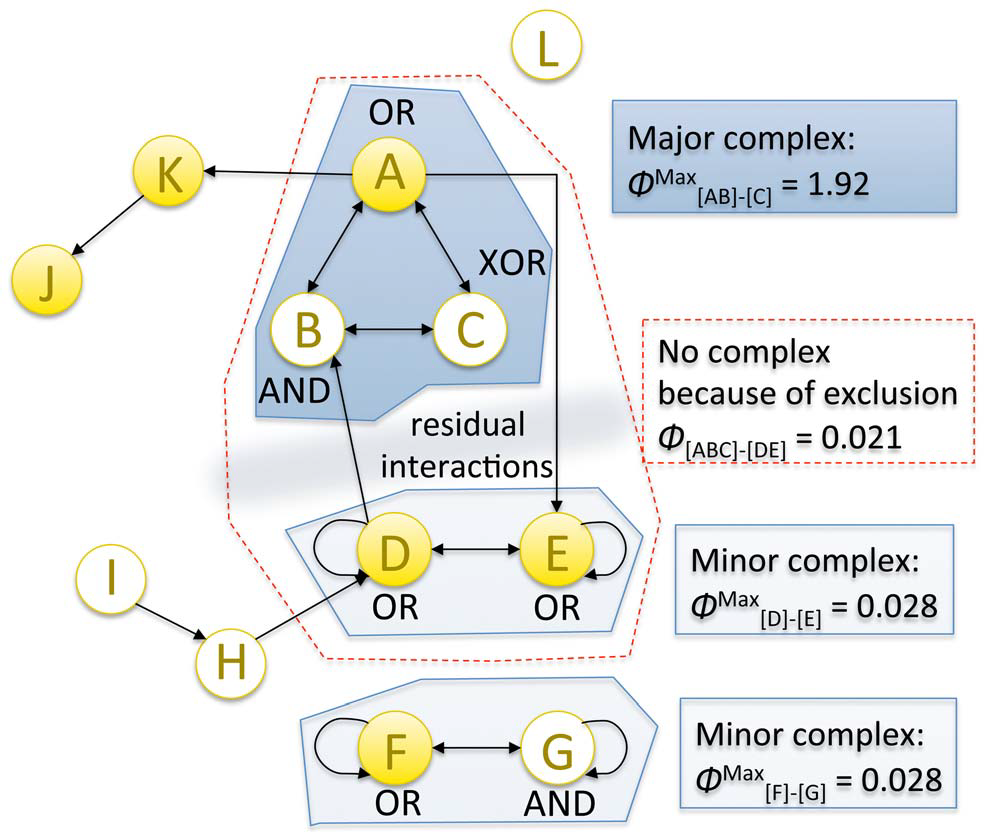
\includegraphics[width=\textwidth]{several}
				\end{figure}
			\end{column}
		\end{columns}
		
	\end{frame}
				
	\begin{frame}
		\frametitle{Приложения и выводы}
		
		Тип связей определяет уровень сознания: мозжечок (A), кора (C), сон или анестезия (B). 
		\begin{figure}
			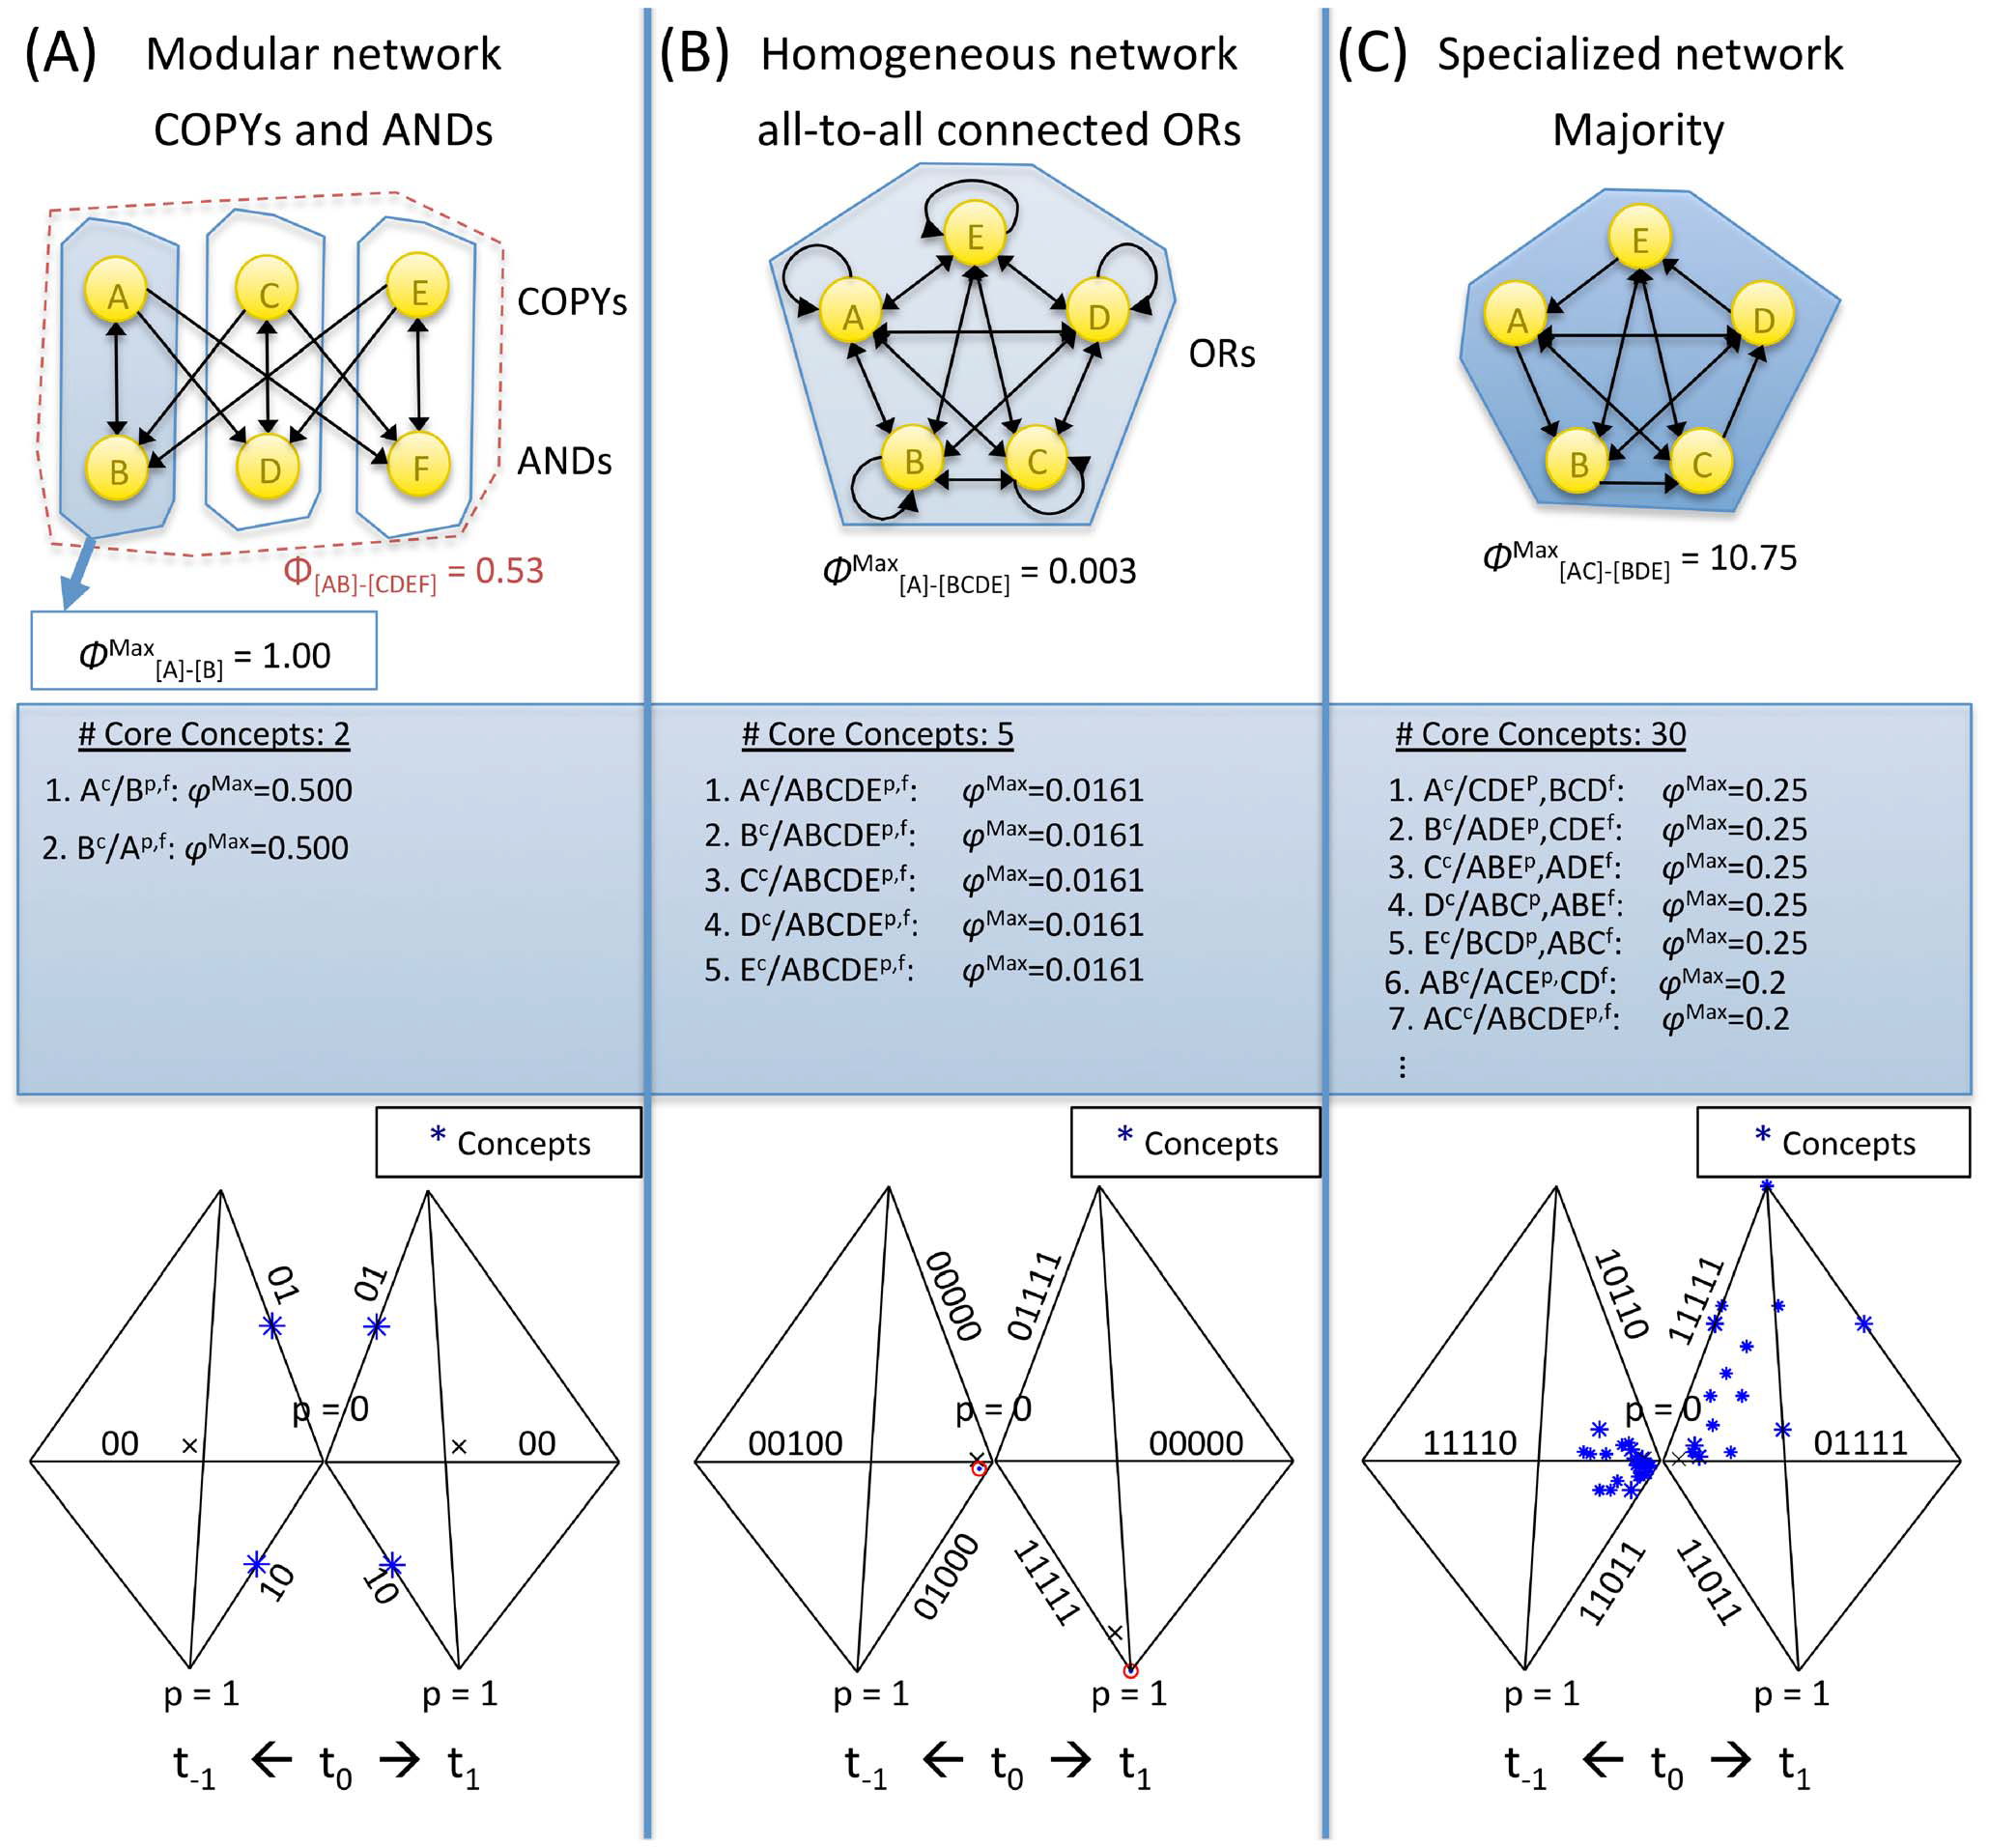
\includegraphics[width=0.6\textwidth]{networks}
		\end{figure}
	\end{frame}
					
	\begin{frame}
		\frametitle{Приложения и выводы}
		
		Неактивная система может быть осознанной, т.к. и активные и неактивные элементы вносят вклад в концептуальную структуру (доминантный комплекс только из неактивных нейронов!).
		\begin{figure}
			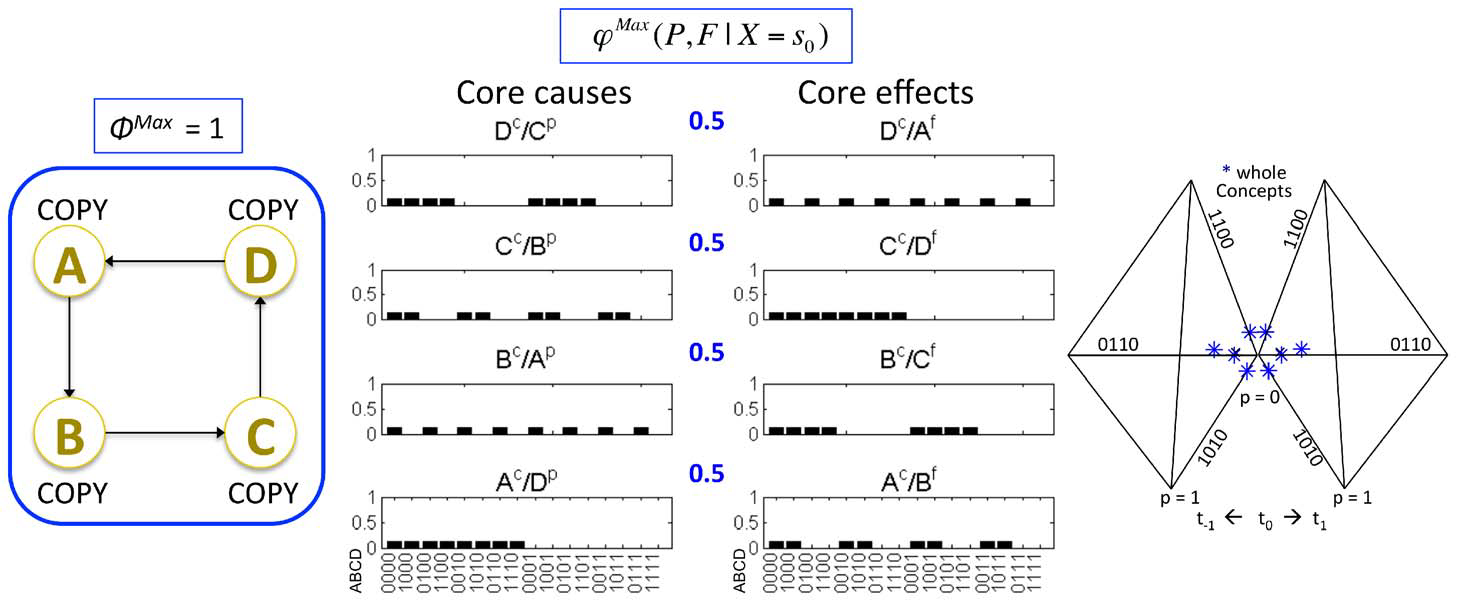
\includegraphics[width=0.8\textwidth]{nonactive}
		\end{figure}
	\end{frame}

	\begin{frame}
		\frametitle{Приложения и выводы}
		
		Даже простые системы обладают сознанием: <<минимально осознанный>> фотодиод.
		\begin{figure}
			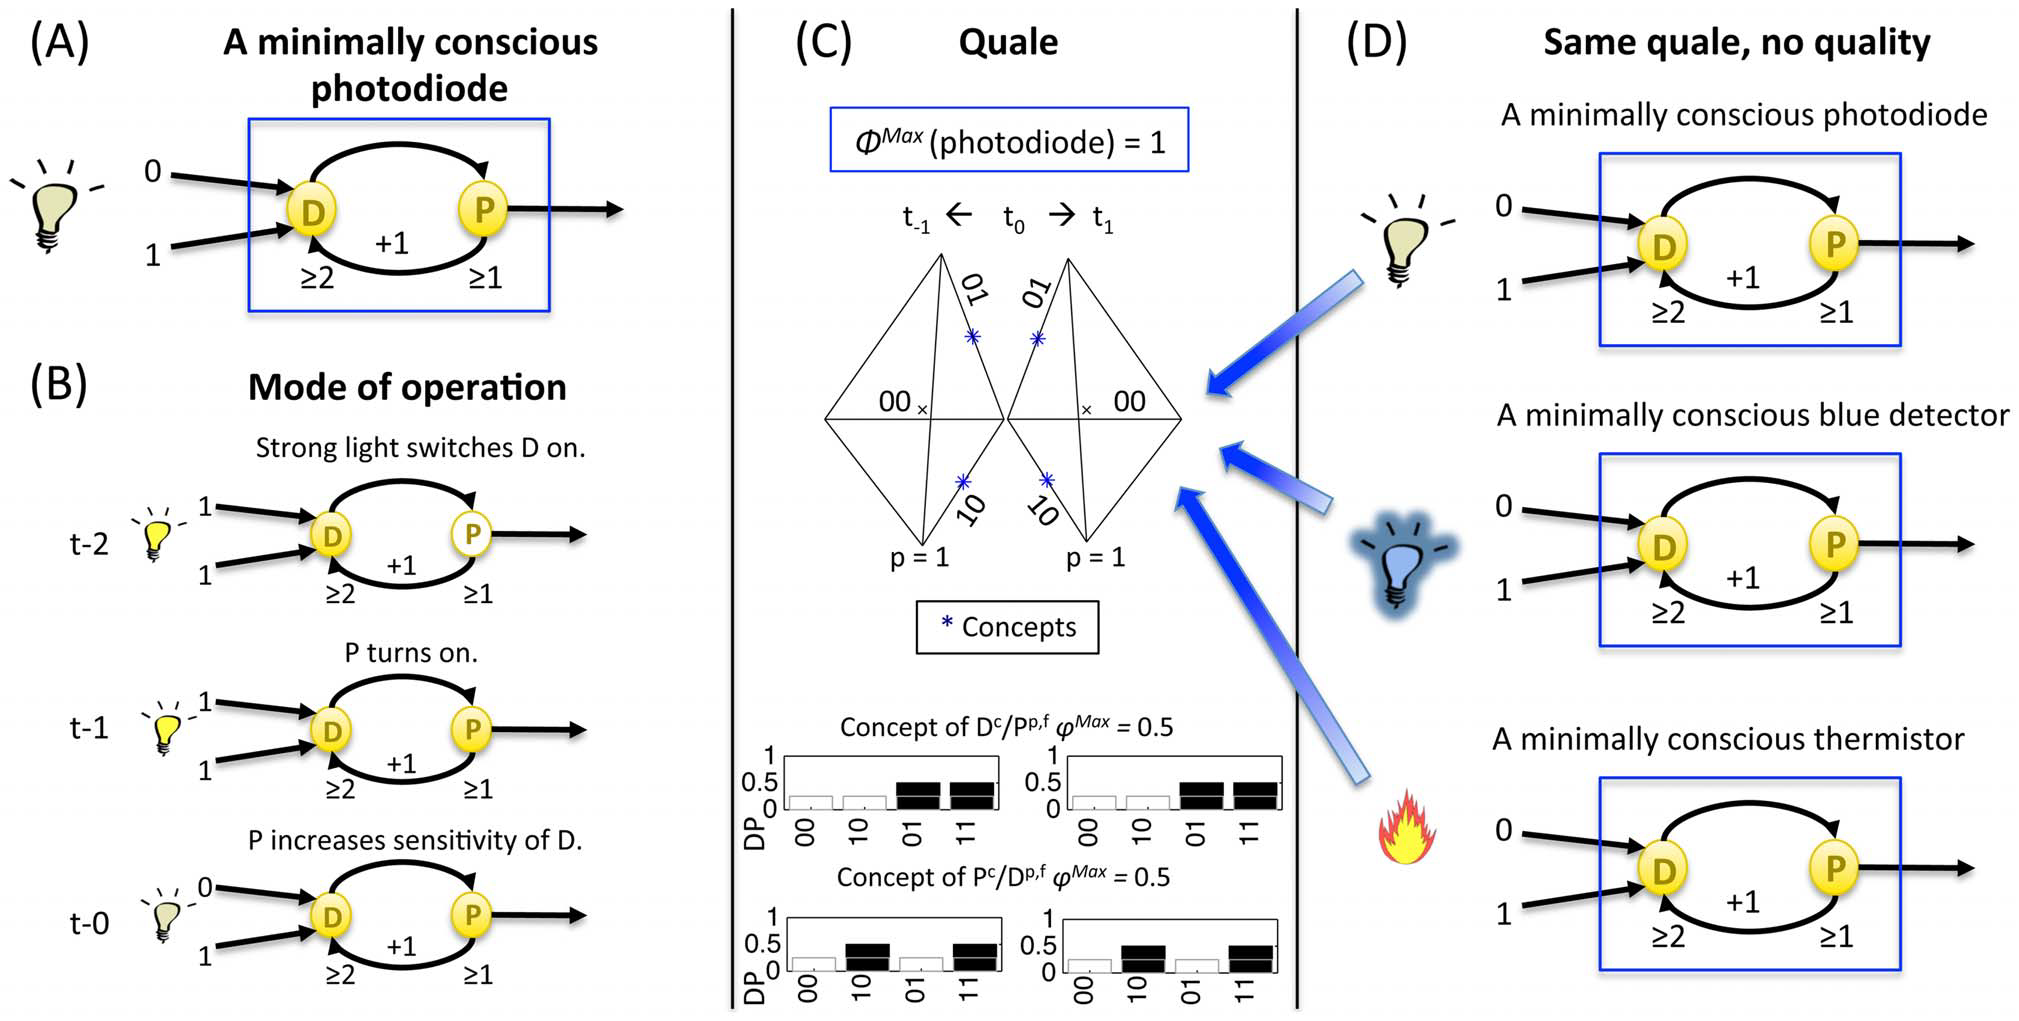
\includegraphics[width=\textwidth]{photod}
		\end{figure}
	\end{frame}

	\begin{frame}
		\frametitle{Приложения и выводы}
		
		Даже сложные системы могут не обладать сознанием: реактивная <<зомби>>-сеть. Важна рекурсия, обратная связь, повторный вход, но только их не достаточно.
		\begin{figure}
			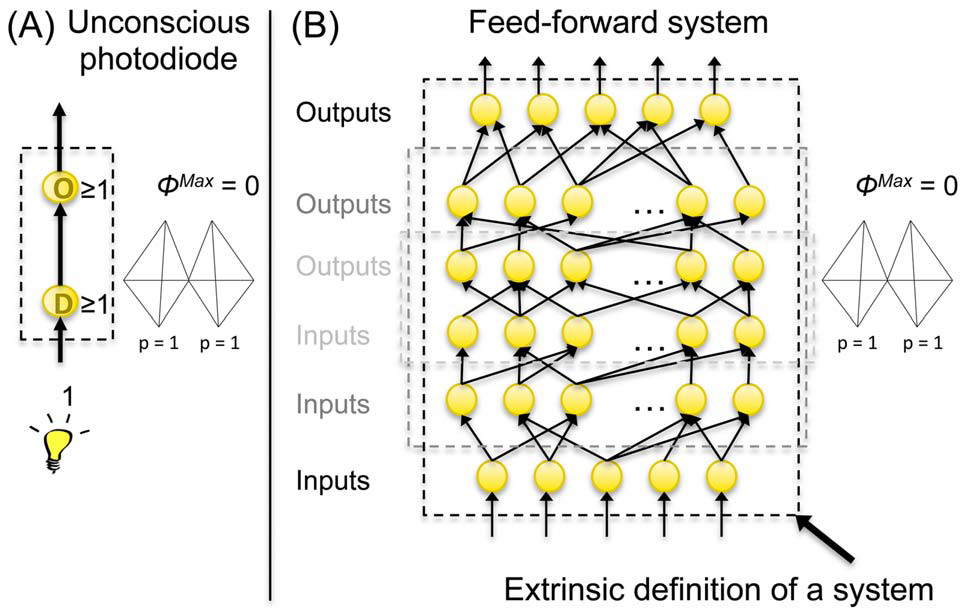
\includegraphics[width=0.8\textwidth]{feedforw}
		\end{figure}
	\end{frame}

	\begin{frame}
		\frametitle{Приложения и выводы}
		
		Сознательная сложная система и бессознательная <<зомби>>-система могут быть функционально эквивалентны. Осознанность нельзя определить только по внешним проявлениям.
		\begin{figure}
			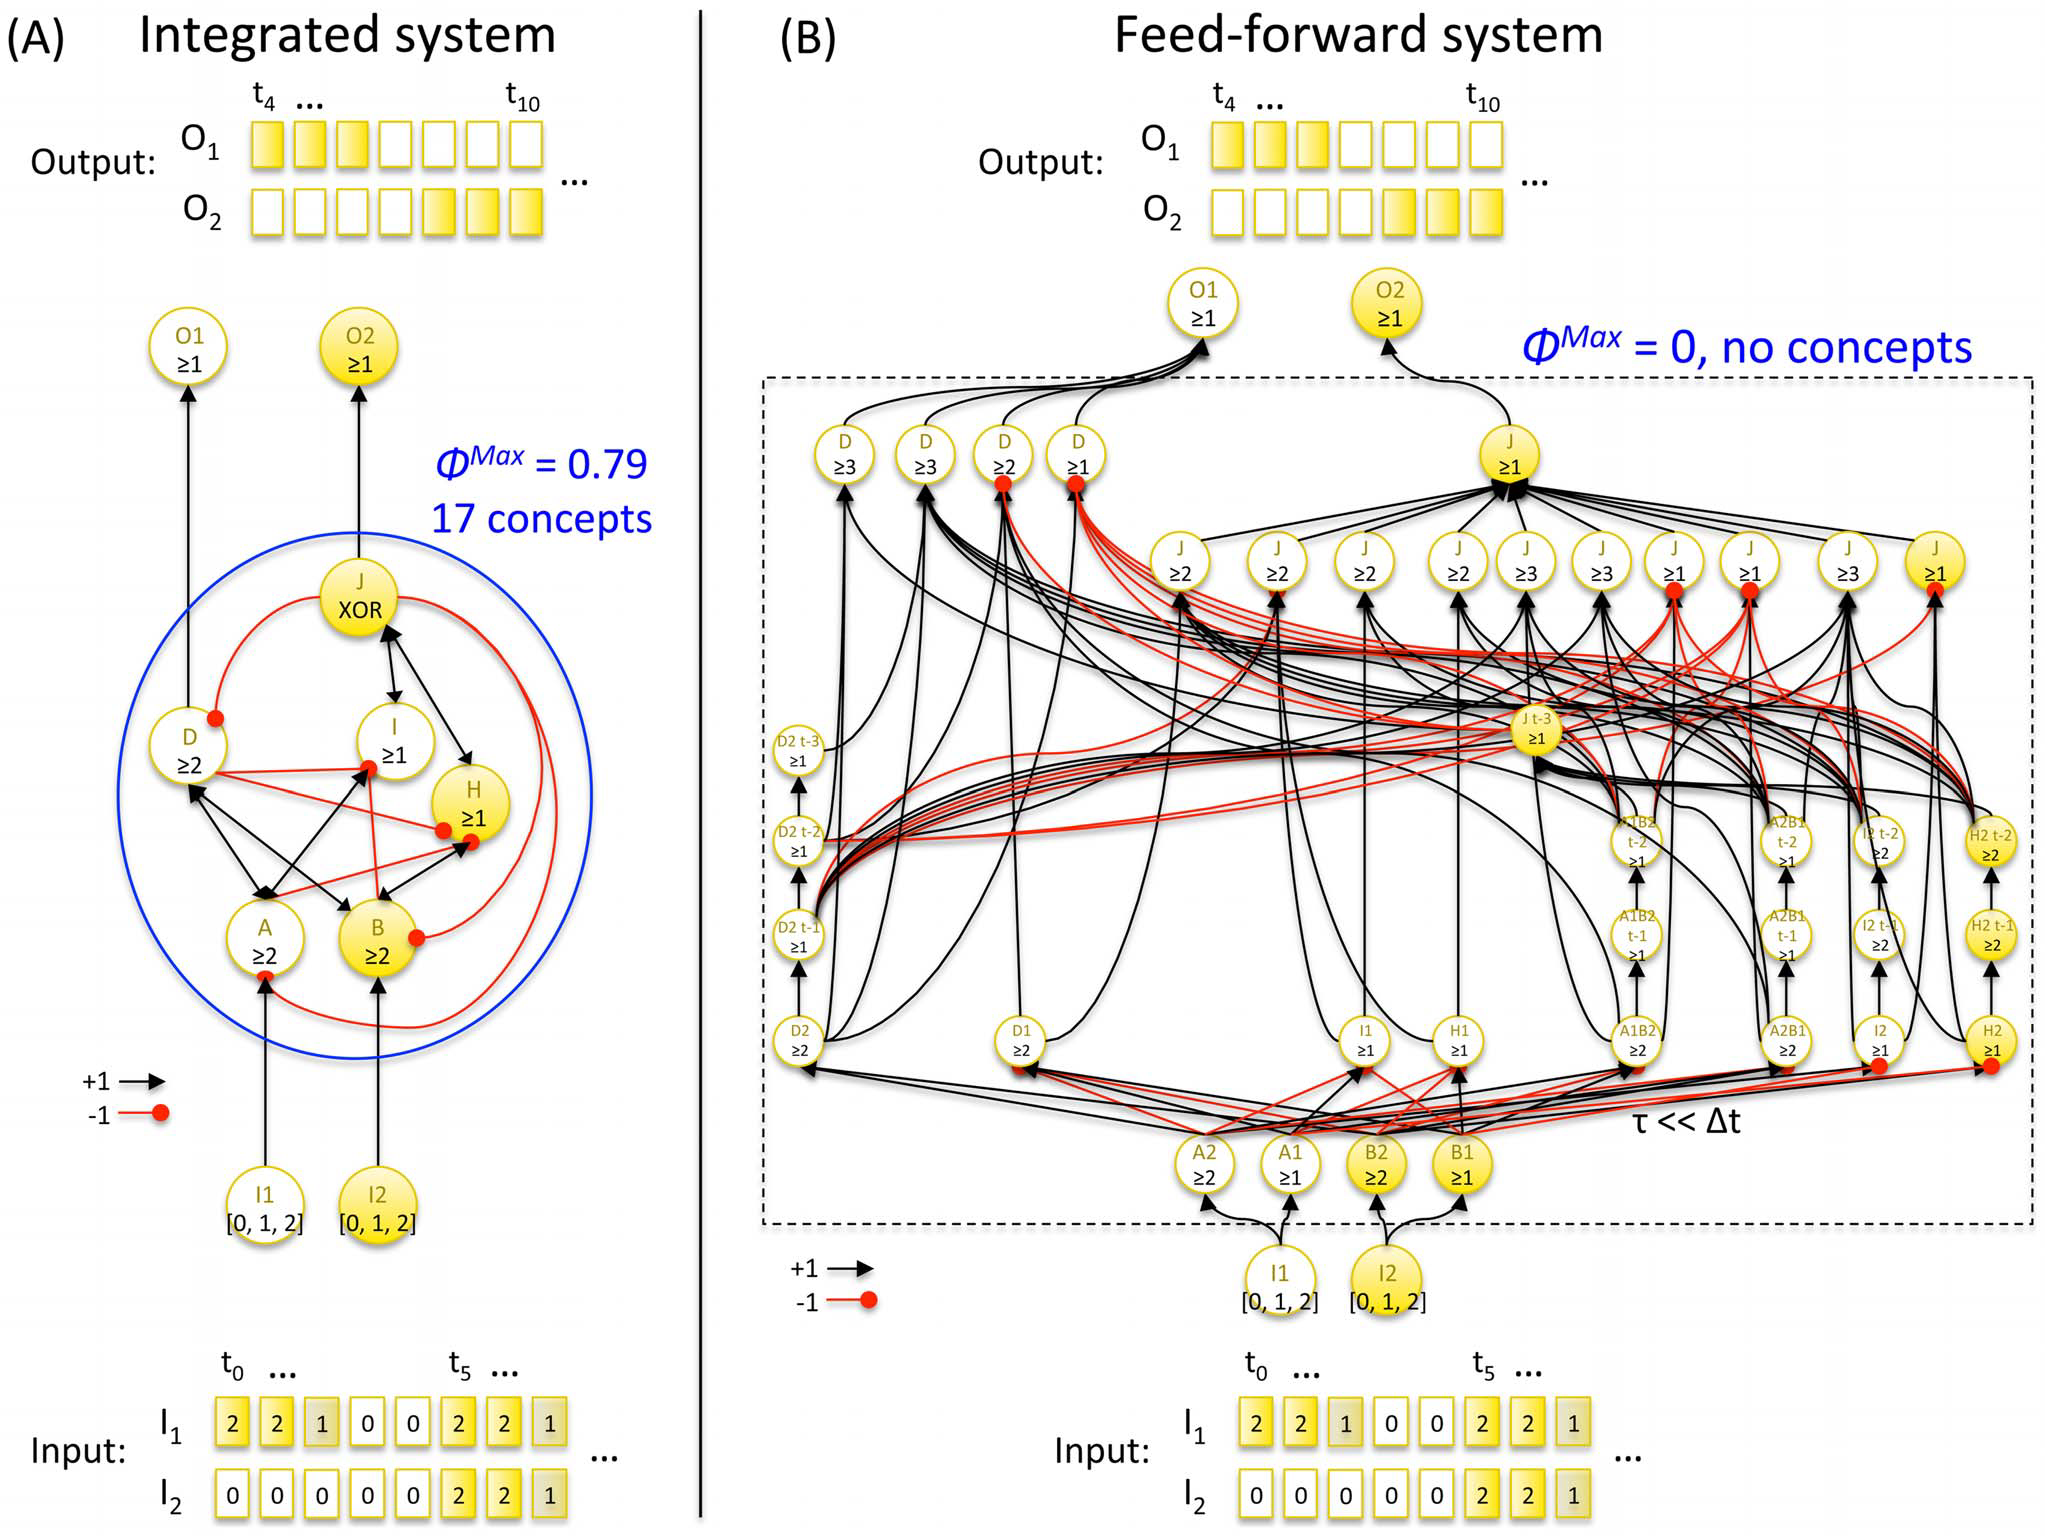
\includegraphics[width=0.65\textwidth]{equals}
		\end{figure}
	\end{frame}
				
	\begin{frame}
		\frametitle{Ограничения и неполнота теории}
		
		Данный подход применить для моделирования реальной физической системы (мозга) невозможно:
		\begin{itemize}
			\item необходимо либо дискретизировать интересующие перемененные или расширять модель до непрерывных значений,
			\item для биологических систем очень немного наблюдаемых состояний,
			\item высокая вычислительная сложность уже при более 12 элементов.
		\end{itemize}

		Необходимо уточнить следующие моменты:		
		\begin{itemize}
			\item не обсуждалась связь MISC и ощущений разной модальности,
			\item необходимо вычислять пространственно-временное разрешение, а не задавать его заранее оптимальным,
			\item не обсуждалось как значение комплекса задается через MICS,
			\item не обсуждается соотнесение внешней каузальной структуры внешней среды и внутренней каузальной структуры MICS (повышение осознанности при адаптации к внешней среде),
			\item гипотеза о том, что интегрированная информация и каузальность одно и то же, требует уточнения.
		\end{itemize}
	\end{frame}
														
%	\begin{frame}
%		\frametitle{Цели курса}
%		
%		\begin{columns}
%			\begin{column}{0.5\textwidth}
%				
%			\end{column}
%			\begin{column}{0.5\textwidth}
%				\begin{figure}
%					
\includegraphics[width=\textwidth]{logo}
%				\end{figure}
%			\end{column}
%		\end{columns}
%	\end{frame}
	%	\begin{frame}
	%		\frametitle{Цели курса}
	%		
	%		\begin{itemize}
	%			\item
	%		\end{itemize}
	%	\end{frame}
	
\end{document}
	
	
